% Copyright 2009--2010  Ed Bueler

%\documentclass[10pt,hyperref={pdfpagelabels=false}]{beamer}
\documentclass[10pt]{beamer}

\mode<presentation>
{
  \usetheme{Hannover}
  % or ...

  \usecolortheme{crane}

  \setbeamercovered{transparent}
  % or whatever (possibly just delete it)
  
  \setbeamerfont{frametitle}{size=\large}
}

\usepackage[english]{babel}
\usepackage[latin1]{inputenc}
\usepackage{times}
\usepackage[T1]{fontenc}
% Or whatever. Note that the encoding and the font should match. If T1
% does not look nice, try deleting the line with the fontenc.

\usepackage{empheq}
\usepackage{amsmath}
\usepackage{esint}
\usepackage{animate}
\usepackage{xspace}
\usepackage{verbatim}
\usepackage{hyperref}

% we can generate a reference list if bibtex is applied to this .tex,
%   and here's the style:
\usepackage{natbib}


\title[Numerical modelling]{
Numerical modelling \\ 
of ice sheets and ice shelves}

\author{Ed Bueler}

\institute{
Dept of Mathematics and Statistics \\
and Geophysical Institute \\
University of Alaska, Fairbanks}

\lecture[1]{Numerical modelling of ice sheets and ice shelves}{lecture-text}


\date{September 2010 \\ Karthaus Summer School}


% remove this when printing out:
\AtBeginSection[]
{
  \begin{frame}<beamer>
    \frametitle{Outline}
    \tableofcontents[currentsection,hideallsubsections]
  \end{frame}
}


% If you wish to uncover everything in a step-wise fashion, uncomment:
%\beamerdefaultoverlayspecification{<+->}

\newcommand{\bg}{\mathbf{g}}
\newcommand{\bq}{\mathbf{q}}
\newcommand{\bu}{\mathbf{u}}
\newcommand{\bw}{\mathbf{w}}

\newcommand{\bA}{\mathbf{A}}
\newcommand{\bbF}{\mathbf{F}}
\newcommand{\bU}{\mathbf{U}}

\newcommand{\ddt}[1]{\ensuremath{\frac{\partial #1}{\partial t}}}
\newcommand{\ddx}[1]{\ensuremath{\frac{\partial #1}{\partial x}}}
\newcommand{\ddy}[1]{\ensuremath{\frac{\partial #1}{\partial y}}}
\newcommand{\pp}[2]{\ensuremath{\frac{\partial #1}{\partial #2}}}
\renewcommand{\t}[1]{\texttt{#1}}
\newcommand{\eps}{\epsilon}
\newcommand{\grad}{\nabla}
\newcommand{\Div}{\nabla\cdot}
\newcommand{\strainrate}{D}
\newcommand{\devstress}{\tau}

\newcommand{\Matlab}{\textsc{Matlab}\xspace}
\newcommand{\Octave}{\textsc{Octave}\xspace}

\newcommand{\exer}[2]{\medskip\noindent \textbf{#1.}\quad #2}
\mode<presentation>{
\newcommand{\slidepage}[1]{slide \pageref{#1}}
}

\newcommand{\mname}[1]{\href{http://www.dms.uaf.edu/~bueler/karthaus/mfiles/#1}{\texttt{#1}}}

\newcommand{\txtinput}[1]{ \scriptsize \verbatiminput{#1} }

\newcommand{\txtinputtiny}[1]{ \tiny \verbatiminput{#1} }

\newcommand{\mmessage}[1]{\begin{center}
\emph{see code} \url{http://www.dms.uaf.edu/~bueler/karthaus/mfiles/#1.m}
\end{center}}

\newcommand{\mmess}[1]{\vspace{-0.1in}\begin{center}
\fbox{\url{http://www.dms.uaf.edu/~bueler/karthaus/mfiles/#1.m}}
\end{center}}


\newcommand{\minput}[1]{
\scriptsize \verbatiminput{mfiles/#1.slim.m}
\vspace{-0.2in}
\tiny \mmess{#1}
\normalsize
}


\newcommand{\minputtiny}[1]{
\tiny \verbatiminput{mfiles/#1.slim.m}
\vspace{-0.16in}
\mmess{#1}
\normalsize
}


\begin{document}

\begin{frame}
  \maketitle
\end{frame}

% the major parts are in separate files:

% Copyright 2009--2010  Ed Bueler

\begin{frame}{notation} 

\begin{center}
  \includegraphics[width=0.8\textwidth]{photos/flowline}

\vspace{-0.1in}
\tiny \emph{figure modified from} [Schoof, 2007]\nocite{SchoofMarine1} \normalsize
\end{center}

\scriptsize
  \begin{itemize}
  \item coordinates $t,x,y,z$ \hfill  ($z$ is vertical, positive upward)
  \item subscripts for partial derivatives: $u_x = \partial u/\partial x$
  \item $h=$ ice surface elevation, \quad $b=$ bedrock elevation
  \item $H=$ ice thickness
  \item $T=$ ice temperature
  \item $(u,v,w)=$ ice velocity
  \item $\rho=$ density of ice, \quad $\rho_w=$ density of ocean water
  \item $g=$ acceleration of gravity
  \item $\strainrate_{ij}=$ strain rate tensor
  \item stress tensors: $\sigma_{ij}=$ Cauchy and $\tau_{ij}=$ deviatoric
  \item \alert{please ask about notation!} \qquad \scriptsize \dots there are no stupid questions \small
  \end{itemize}

\emph{notation here is generally consistent with  [Bueler and others, 2005]\nocite{BLKCB}, [Bueler and Brown, 2009]\nocite{BBssasliding}, [Fowler, 1997]\nocite{Fowler}, [Greve and Blatter, 2009]\nocite{GreveBlatter2009}, [Schoof, 2006; 2007]\nocite{SchoofStream,SchoofMarine1}}
\end{frame}


\begin{frame}{scope}

slogans:
  \begin{itemize}
  \item \alert{my focus is on approximating ice flow}
  \item \alert{my example numerical codes actually work}
  \end{itemize}
\medskip

continuum models:
  \begin{itemize}
  \item shallow ice approximation (SIA) in 2D
  \item shallow shelf approximation (SSA) in flowline (1D)
  \item mass continuity \& surface/base kinematical equations
  \item \dots and a little bit more
  \end{itemize}

\medskip
numerical ideas:
  \begin{itemize}
  \item finite difference schemes
  \item solving algebraic systems arising in stress balances
  \item verification
  \end{itemize}
\end{frame}


\begin{frame}{outside of scope}
\large\emph{not} \normalsize covered here:
  \begin{itemize}
  \item thermomechanical coupling
  \item subglacial material/process modeling
  \item snow/firn process modeling
  \item earth deformation
  \item numerical solution of Stokes equations
  \item grounding line and calving front issues
  \item anisotropy in ice flow
  \item paleoclimate modeling and ``spin-up''
  \item finite element, spectral, wavelet, multigrid, \dots methods
  \item \dots etc.~etc.
  \end{itemize}
\end{frame}


\begin{frame}{main equations}

\begin{itemize}
\item shallow ice approximation (SIA), equation \eqref{sia}
\item heat equation \eqref{heat} \quad\small\emph{(for analogy purposes)} \normalsize
\item surface kinematical equation \eqref{surfkine}
\item basal kinematical equation \eqref{basekine}
\item map-plane mass continuity equation \eqref{masscontinuity}
\item Stokes equations in a flow line, equations \eqref{Stokes}
\item shallow shelf approximation (SSA), equation \eqref{ssa}
\end{itemize}
\end{frame}


\begin{frame}{\textsc{Matlab}/\textsc{Octave} codes}

\begin{itemize}
\item these lectures are structured around
  \begin{itemize}
    \item 7 codes which solve PDEs
    \item an additional 13 codes which plot, pre-process, post-process
  \end{itemize}
\item \emph{each PDE code is 1/2 to 1 page in length}
\item all tested in \Matlab \scriptsize(v.~7.9) \normalsize and \href{http://www.gnu.org/software/octave/}{\Octave} \scriptsize(v.~3.2)\normalsize
\item available as
  \begin{itemize}
    \item[$\circ$] \texttt{.zip} or \texttt{.tar.gz}, from my USB memory stick, or
    \item[$\circ$] online:  \bigskip\small
      \centerline{\fbox{\url{http://www.dms.uaf.edu/~bueler/karthaus/}}}
  \end{itemize}
\end{itemize}
\end{frame}


\section[ice flow: a superficial view]{ice flow: an outsider's superficial view}

\begin{frame}{my first goal}

\begin{itemize}
\item I want to get to an equation for which I can say:
\bigskip

\begin{center}
\emph{numerically solve this equation, and you've got a usable model for} \dots (a specific ice flow problem) 
\end{center}
\bigskip

\item to get to that goal: I will \emph{very quickly} recall the continuum mechanics of ice flow
\item \dots from a naive outside view
\end{itemize}
\end{frame}


\begin{frame}{let's treat ice in glaciers as a \emph{fluid}}

\begin{itemize}
\item we describe fluids primarily by a \emph{velocity field} $\mathbf{u}(t,x,y,z)$
\item if the ice fluid were much faster-moving than it actually is\footnote{if gravity were a lot stronger and/or ice were a lot weaker, for example}, and if it were linearly-viscous like liquid water, then ice flow modeling would be more familiar to other the climate-modeling and/or engineering computational fluids people
\item \dots we would all use the Navier-Stokes equations, for incompressible fluids, as our flow model:
\begin{align*}
\nabla \cdot \mathbf{u} &= 0 &&\text{\emph{incompressibility}} \\
\rho \left(\mathbf{u}_t + \mathbf{u}\cdot\nabla \mathbf{u}\right) &= -\nabla p + \nu \nabla^2 \mathbf{u} + \rho \mathbf{g} &&\text{\emph{force balance}}
\end{align*}
\end{itemize}
\end{frame}


\begin{frame}{\emph{hmmm} \dots \emph{does not sound like glaciology to me!}}

is numerical ice flow modeling actually computational fluid dynamics?

\begin{itemize}
\item \alert{yes}
\item at geophysical scale like atmosphere/ocean
\item \dots but it is a weird one
\item consider what makes atmosphere/ocean flow modeling exciting:
  \begin{itemize}
  \item[$\circ$] turbulence
  \item[$\circ$] convection
  \item[$\circ$] coriolis force
  \item[$\circ$] density/salinity stratification
  \item[$\circ$] lots of tracers \& chemistry ($CO_2$, methane, ozone, \dots)
  \end{itemize}
\item none of the above list is relevant to ice flow!
\item so what could be interesting about the flow of slow, cold, shallow, non-turbulent, chemically-dull, old ice?
\end{itemize}
\end{frame}


\begin{frame}{ice is a slow, shear-thinning fluid}

\begin{itemize}
\item our fluid is

\phantom{foo bar}
  \begin{tabular}{lc}
  \emph{slow}: & $\rho \left(\mathbf{u}_t + \mathbf{u}\cdot\nabla \mathbf{u}\right) \approx 0$ \\
  \emph{non-Newtonian}: & viscosity $\nu$ is not constant in ``$\tau_{ij} = 2 \nu D_{ij}$''
  \end{tabular}
\item and so the standard ``full'' model for ice flow is shear-thinning Stokes as follows:
\begin{align*}
\nabla \cdot \mathbf{u} &= 0 &&\text{\emph{incompressibility}} \\
0 &= - \nabla p + \nabla \cdot \tau_{ij} + \rho \mathbf{g} &&\text{\emph{force balance}} \\
D_{ij} &= A \tau^{n-1} \tau_{ij} &&\text{\emph{flow law}}
\end{align*}
\item equations above are true at every instant, and so
  \begin{quote}
  \emph{geometry and boundary stress and ice strength determine velocity instantaneously} in the model
  \end{quote}
\end{itemize}
\end{frame}


\begin{frame}{ice is a slow fluid 2}

\begin{itemize}
\item the ``slow'' fact, $\rho \left(\mathbf{u}_t + \mathbf{u}\cdot\nabla \mathbf{u}\right) \approx 0$, means no forces of inertia from acceleration
\item thus velocity is \emph{not} a state variable of any model for evolving ice sheets and glaciers
\item \dots it is a ``diagnostic'' output \dots but a very important output!
\item an ice sheet code usually recomputes the full velocity field at every time, without storing it from the previous step\footnote{Bob Dylan would say: \emph{you don't need a glaciologist to remember which way the wind blows}}
\item to see how glacier flow fields change in time we must track the changes to
  \begin{itemize}
    \item[$\circ$] the location of the ice surface and base
    \item[$\circ$] the force (stress) applied at the boundary
    \item[$\circ$] the ice strength, as it changes with ice temperature (for example)
  \end{itemize}
\end{itemize}
\end{frame}


\begin{frame}{plane flow Stokes}

more concretely, the shear-thinning Stokes model is this:

\begin{itemize}
\item in the $x,z$ plane flow case the Stokes equations say
\begin{empheq}[]{align}
u_x + w_z &= 0 &&\text{\emph{incompressibility}}\notag \\
p_x &= \tau_{11,x} + \tau_{13,z} &&\text{\emph{stress balance} ($x$)} \notag \\
p_z &= \tau_{13,x} - \tau_{11,z} - \rho g &&\text{\emph{stress balance} ($z$)} \notag \\
u_x &= A \tau^{n-1} \tau_{11} &&\text{\emph{flow law} (diagonal)}\notag \\
u_z + w _x &= 2 A \tau^{n-1} \tau_{13} &&\text{\emph{flow law} (off-diagonal)} \notag
\end{empheq}
\item five equations in five unknowns ($u,w,p,\tau_{11},\tau_{13}$)
\item complicated enough \dots can I make it familiar by looking at a very-simplified situation?
\end{itemize}
\end{frame}


\begin{frame}{slab-on-a-slope}

\vspace{-0.05in}
\small

\begin{columns}
\begin{column}{0.5\textwidth}
\begin{itemize}
\item rotated coordinates: $\mathbf{g} = g \sin\theta\, \hat x - g \cos \theta \,\hat z$
\end{itemize}
\end{column}
\begin{column}{0.5\textwidth}
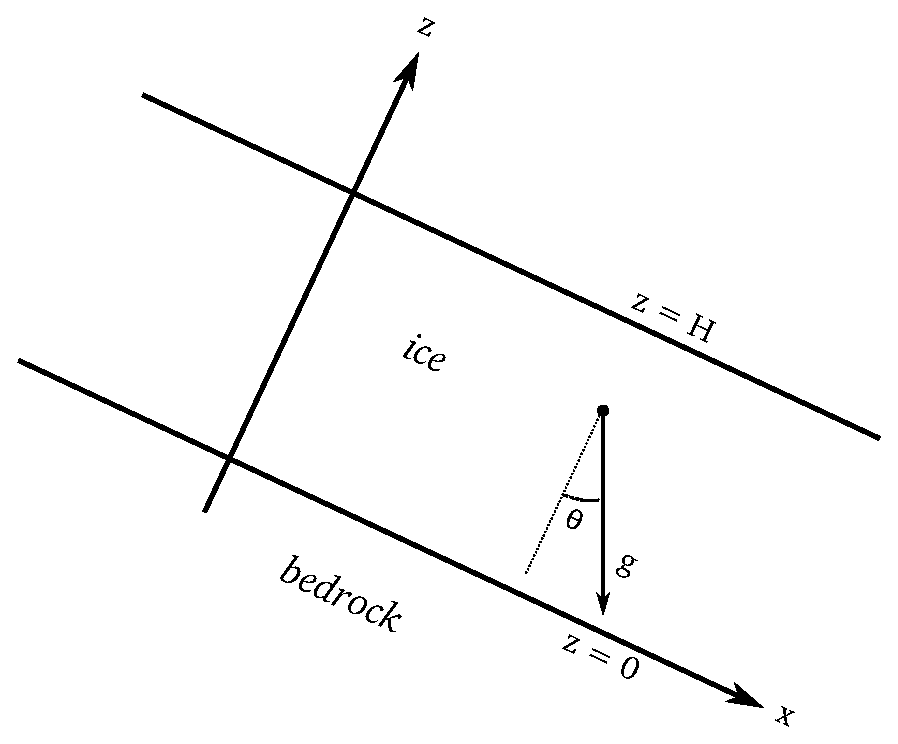
\includegraphics[width=1.0\textwidth]{photos/slab}
\end{column}
\end{columns}
\vspace{-0.2in}

\begin{itemize}
\item as on previous slide, but with $n=3$:
\small
\begin{empheq}[]{align}
u_x + w_z &= 0 &   u_x &= A \tau^2 \tau_{11} \notag \\
p_x &= \tau_{11,x} + \tau_{13,z} + \rho g \sin\theta &   u_z + w _x &= 2 A \tau^2 \tau_{13} \notag \\
p_z &= \tau_{13,x} - \tau_{11,z} - \rho g \cos\theta \notag
\end{empheq}
\small
\item \emph{but} for a slab-on-a-slope, by definition, there is no variation in $x$:
\small
\begin{empheq}[]{align}
w_z &= 0 &   0 &= \tau_{11} \notag \\
\tau_{13,z} &= - \rho g \sin\theta &   u_z &= 2 A \tau^2 \tau_{13} \notag \\
p_z &= - \rho g \cos\theta \notag
\end{empheq}
\end{itemize}
\end{frame}


\begin{frame}{slab-on-a-slope 2}

\small
\begin{itemize}
\item add some boundary conditions:
	$$w(\text{base})=0, \qquad p(\text{surface})=0, \qquad u(\text{base})=u_0,$$
\item further-simplified equations:
\begin{align*}
\tau_{13} &= \rho g \sin\theta (H-z) &  p &= \rho g \cos\theta (H-z) \\
w &= 0  & \tau_{11} &= 0
\end{align*}
\item and 
\vspace{-0.2in}
\begin{align*}
u(z) &= u_0 + 2 A (\rho g \sin\theta)^3 \int_0^z (H-z')^3\,dz' \\
     &= u_0 + \frac{1}{2} A (\rho g \sin\theta)^3  \left(H^4 - (H-z)^4\right)
\end{align*}

\vspace{-0.1in}
\end{itemize}
\begin{center}
\includegraphics[width=0.6\textwidth]{photos/slabfigs}
\end{center}
\end{frame}


\begin{frame}{slab-on-a-slope 3}

\begin{columns}
\begin{column}{0.6\textwidth}
\begin{itemize}
\item do we believe these equations?
\item velocity on last slide (and below) was from a \emph{formula}
\item compare to observations at right
\item seems there is an element of truth
\end{itemize}
\begin{center}
\includegraphics[width=0.4\textwidth]{photos/slabvel}
\end{center}
\end{column}
\begin{column}{0.4\textwidth}
\includegraphics[width=0.9\textwidth]{photos/athabasca_deform}

\medskip
\scriptsize
Velocity profile of the Athabasca Glacier, Canada, derived from inclinometry.  [Savage and Paterson, 1963]\nocite{SavagePaterson}
\end{column}
\end{columns}
\end{frame}


\begin{frame}{mass continuity}

\small
now we know the velocity $u(z)$ \dots so what?
\begin{itemize}
\item suppose now that our slab has \emph{slowly varying thickness} $H(t,x)$
\item compute the vertical average of velocity, which depends on $x$:
	$$\bar u(x) = \frac{1}{H}\int_0^{H} u(x,z)\,dz$$
\end{itemize}

\begin{columns}
\begin{column}{0.6\textwidth}
\begin{itemize}
\item consider change of area (really: ice volume) in the figure at right:
	$$\frac{dA}{dt} = \int_{x_1}^{x_2} M(x)\,dx + \bar u_1 H_1 - \bar u_2 H_2$$
\item in limit where width $dx=x_2-x_2$ is small we have $A\approx dx\, H$
\item divide by $dx$ and get
   $$H_t = M - \left(\bar u H\right)_x$$
\item this is the \emph{mass continuity equation}
\end{itemize}
\end{column}
\begin{column}{0.4\textwidth}
\includegraphics[width=1.0\textwidth]{photos/slabmasscontfig}
\end{column}
\end{columns}
\end{frame}


\begin{frame}{rough explanation of ``shallow ice approximation'' (SIA)}

\small
\begin{itemize}
\item I'll consider only $u_0=0$ case in these lectures (``non-sliding SIA'')
\item from slab-on-slope velocity formula,
\begin{align*}
\bar u H &= \int_0^H \frac{1}{2} A (\rho g \sin\theta)^3  \left(H^4 - (H-z)^4\right)\,dz \\
	&= \frac{1}{2} A (\rho g \sin\theta)^3  \left(\frac{4}{5} H^5\right) \\
	&= \frac{2}{5} A (\rho g \sin\theta)^3 H^5
\end{align*}
\item note $\sin \theta \approx \tan\theta = - h_x$
\item combine with mass continuity $H_t = M - \left(\bar u H\right)_x$:
\begin{equation}
H_t = M + \left(\frac{2}{5} A (\rho g)^3 H^5 |h_x|^2 h_x\right)_x  \tag{0}
\end{equation}
\item \emph{it is pretty rough \dots but we will get back to it}
\end{itemize}
\end{frame}


\begin{frame}{slow, non-Newtonian, shallow}

\begin{itemize}
\item ice sheet flow problems have three outstanding properties:
  \begin{enumerate}
  \item slow
  \item non-Newtonian
  \item shallow
  \end{enumerate}
\item all three properties will be in all of my models
\item regarding ``shallow,'' here in \alert{red} is a to-scale cross section of Greenland at $71^\circ$:
\begin{center}
  \includegraphics[width=0.6\textwidth]{photos/green_transect}
\end{center}
\end{itemize}
\end{frame}


\subsection{shallow ice approximation (SIA)}

\begin{frame}{the isothermal shallow ice approximation (SIA)}

is a model which applies reasonably well to
\begin{itemize}
\item grounded ice sheets
\item on relatively uninteresting bed topography, whose flow is
\item not dominated by sliding nor by liquid water at base or margin
\begin{center}
  \includegraphics[width=0.7\textwidth]{photos/polaris}

\tiny ``Polaris Glacier,'' northwest Greenland, photo 122, [Post and LaChapelle, 2000]\nocite{PostLaChapelle}
\end{center}
\item might apply to the above
\end{itemize}
\end{frame}


\begin{frame}{isothermal shallow ice approximation 2}

\begin{itemize}
\item the non-sliding isothermal SIA:
\begin{empheq}[box=\fbox]{equation}
H_t = M + \Div \left(\Gamma H^{n+2} |\grad h|^{n-1} \grad h \right) \label{sia}
\end{empheq}
  \begin{itemize}
  \item[$\circ$] generalizes slab-on-slope equation (0) earlier
  \item[$\circ$] $h=H+b$
  \item[$\circ$] accumulation if $M>0$, ablation if $M<0$
  \item[$\circ$] recall Glen flow law: $\strainrate_{ij} = A(T) \devstress^{n-1} \devstress_{ij}$
  \item[$\circ$] $\Gamma$ is a positive constant
  \end{itemize}
\item \begin{minipage}[t]{2.5in}\emph{numerically solve equation \eqref{sia}, and you have a usable model for ice flow in the Barnes Ice Cap} [Mahaffy, 1976]\nocite{Mahaffy}\end{minipage}
\, \begin{minipage}[t]{1.1in}\vspace{-10pt}\includegraphics[width=1.0in]{photos/barnes}\end{minipage}
\item questions:
  \begin{itemize}
     \item[$\circ$] where does equation \eqref{sia} come from?
     \item[$\circ$] how to solve it numerically?
     \item[$\circ$] how to \emph{think} about it?
  \end{itemize}
\end{itemize}
\end{frame}


% Copyright 2009--2010  Ed Bueler

\section{heat analogy \& numerics}

\subsection{analogy}

\begin{frame}{compare to heat equation}
\label{slide:heatcompare}

\small
\begin{columns}
\begin{column}{0.6\textwidth}
\begin{itemize}
\item recall Newton's law of cooling
	$$\frac{dT}{dt} = -\mu (T-T_{\text{ambient}})$$
where $T$ is temperature and $\mu$ relates to material and geometry of object
\item Newton's law for segments of an insulated rod:
\begin{align*}
\frac{dT_j}{dt} &= -\tilde \mu \left(T_j - \frac{1}{2} (T_{j-1} + T_{j+1}) \right) \\
	&= \frac{\tilde \mu}{2} \left(T_{j-1} - 2 T_j + T_{j+1}\right) 
\end{align*}
(where $\tilde \mu$ is material constant proportional to $\Delta x^{-2}$)
\item this suggests finite difference approximation of a PDE:
	$$T_t = D T_{xx}$$
\end{itemize}
\end{column}
\begin{column}{0.4\textwidth}
\hfill
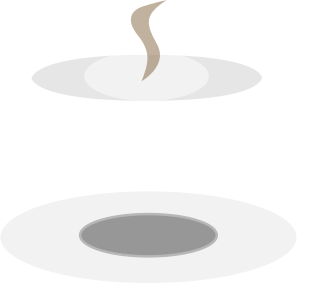
\includegraphics[width=0.5\textwidth]{pdffigs/coffee}
\vspace{0.7in}
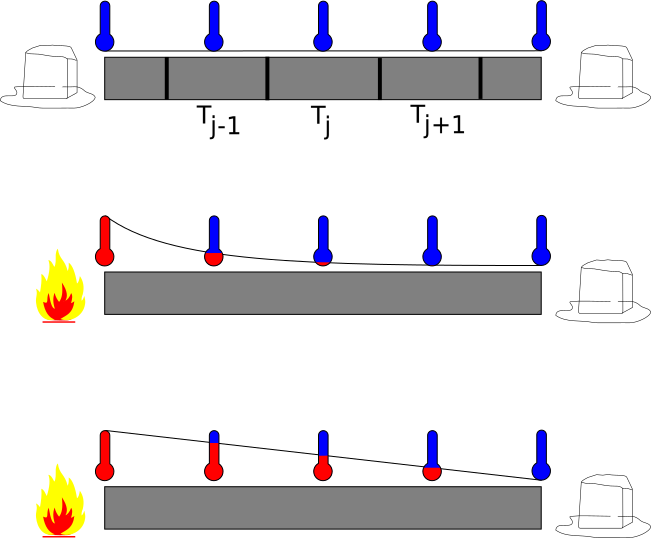
\includegraphics[width=1.0\textwidth]{pdffigs/heatconduction}

%COFFEE: \hfill \tiny (\emph{user:Assassingr, wiki commons image})
%HEAT:  \hfill \tiny (\emph{Christophe Dang Ngoc Chan, wiki commons image})
\end{column}
\end{columns}
\end{frame}


\begin{frame}{compare to heat equation 2}

\small
continuum version:
\begin{columns}
\begin{column}{0.6\textwidth}
\begin{itemize}
\item Fourier rewrote Newton's law as heat flux in continua: $\mathbf{q} = - k \grad u$
\item by conservation of energy, allowing an additional source of heat $f$, get heat equation:
	$$\rho c u_t = f + \Div (k \grad u)$$
\end{itemize}
\end{column}
\begin{column}{0.4\textwidth}
\animategraphics[autoplay,loop,height=2.5cm]{4}{anim/heatmelt}{0}{16}
\end{column}
\end{columns}


\begin{itemize}
\item set $D=k/(\rho c)$ and $M=f/(\rho c)$:
\begin{empheq}[box=\fbox]{equation}
u_t = M + \Div (D\, \grad u) \label{heat}
\end{empheq}
\item this heat equation is a diffusive, time-dependent PDE, \emph{like the SIA model for ice sheets}
\end{itemize}
\end{frame}


\begin{frame}{analogy: SIA versus heat equation}

\begin{itemize}
\item side-by-side comparison:
\begin{center}
\begin{tabular}{cc}
\scriptsize SIA: $H(t,x,y)$ is ice thickness & \scriptsize heat: $u(t,x,y)$ is temperature \normalsize \\
	\boxed{H_t = M + \Div \left({\color{red}\Gamma H^{n+2} |\grad h|^{n-1}}\, \grad h \right)}  &  \boxed{u_t = M + \Div (D\, \grad u)}
\end{tabular}
\end{center}

\medskip
\item we identify the diffusivity in the SIA:
	$$D = {\color{red}\Gamma H^{n+2} |\grad h|^{n-1}}$$
\item non-sliding shallow ice flow \emph{diffuses} the ice because the flow is down the surface gradient

\bigskip
\item some issues with this analogy:
  \begin{itemize}
  \item[$\circ$]  $\grad H\ne \grad h$ when bed is not flat \dots so what?
  \item[$\circ$]  $D$ depends on solution $H(t,x,y)$ \dots how does that complicate the numerical solution method?
  \item[$\circ$]  $D\to 0$ at margin ($H\to 0$) and at dome ($|\grad h|\to 0$) \dots so what?
  \end{itemize}
\item I'll get back to these ``issues'', but now let's get our hands dirty and numerically solve the heat equation
\end{itemize}
\end{frame}


\subsection{finite differences}

\begin{frame}{finite differences for heat equation}

basic ideas of finite differences:
\begin{itemize}
\item for differentiable $f(x)$ and any $\Delta x$, \emph{Taylor} says
\small
	$$f(x+\Delta x) = f(x) + f'(x) \Delta x + \frac{1}{2} f''(x) \Delta x^2 + \frac{1}{3!} f'''(x) \Delta x^3 + \dots$$
\normalsize
\item you can replace ``$\Delta x$'' with other expressions, e.g.:
\small
\begin{align*}
f(x-\Delta x) &= f(x) - f'(x) \Delta x + \frac{1}{2} f''(x) \Delta x^2 - \frac{1}{3!} f'''(x) \Delta x^3 + \dots \\
f(x+2\Delta x) &= f(x) + 2 f'(x) \Delta x + 2 f''(x) \Delta x^2 + \frac{4}{3} f'''(x) \Delta x^3 + \dots
\end{align*}
\normalsize
\item basic finite difference idea for differential equations: \emph{combine expressions like these to approximate derivatives}
\item for all of these notes, grid points have equal spacing $\Delta x$
\end{itemize}
\end{frame}


\begin{frame}{finite differences for heat equation 2}

\begin{itemize}
\item \emph{partial} derivative expressions, for example with $u=u(t,x)$:
\small
\begin{align*}
u_t(t,x) &= \frac{u(t+\Delta t,x) - u(t,x)}{\Delta t} + O(\Delta t), \\
u_t(t,x) &= \frac{u(t+\Delta t,x) - u(t-\Delta t,x)}{2\Delta t} + O(\Delta t^2), \\
u_x(t,x) &= \frac{u(t,x+\Delta x) - u(t,x)}{\Delta x} + O(\Delta x), \\
u_x(t,x) &= \frac{u(t,x+\Delta x) - u(t,x-\Delta x)}{2\Delta x} + O(\Delta x^2), \\
u_{xx}(t,x) &= \frac{u(t,x+\Delta x) - 2 u(t,x) + u(t,x-\Delta x)}{\Delta x^2} + O(\Delta x^2)
\end{align*}
\normalsize
\item sometimes we want a derivative in-between grid points:
\small
	$$u_x(t,x+(\Delta x/2)) = \frac{u(t,x+\Delta x) - u(t,x)}{\Delta x} + O(\Delta x^2)$$
\normalsize
\item ``$+O(\Delta x^2)$'' is better than ``$+O(\Delta x)$'' if $\Delta x$ is a small number
\end{itemize}
\end{frame}


\begin{frame}{explicit scheme for heat equation}
\label{slide:explicit}

\begin{itemize}
\item recall 1D heat equation $u_t = D u_{xx}$
\item the \emph{explicit} scheme using notation $u_j^n \approx u(t_n,x_j)$, so
	$$\frac{u_j^{n+1} - u_j^n}{\Delta t} = D\,\frac{u_{j+1}^n - 2 u_j^n + u_{j-1}^n}{\Delta x^2}$$
\item let $\nu = D \Delta t / (\Delta x)^2$, so
	$$u_j^{n+1} = \nu u_{j+1}^n + (1 - 2 \nu) u_j^n + \nu u_{j-1}^n$$
\end{itemize}

\begin{columns}[b]
\begin{column}{0.70\textwidth}
\begin{itemize}
\item scheme has stencil at right \large $\to$ \normalsize
\item advantage over implicit (later): $u_j^{n+1}$ is determined by \emph{known} quantities at time $t_n$
\bigskip
\end{itemize}
\end{column}
\begin{column}{0.3\textwidth}
\includegraphics[width=1.0\textwidth]{pdffigs/expstencil}
\end{column}
\end{columns}
\end{frame}


\begin{frame}{explicit scheme for heat equation 2}

\begin{itemize}
\item in 2D we write $u_{jk}^n \approx u(t_n,x_j,y_k)$
\item the 2D explicit scheme for the $M=0$ heat equation $u_t = D(u_{xx} + u_{yy})$ is
\small
	$$\frac{u_{jk}^{n+1} - u_{jk}^n}{\Delta t} = D\,\left(\frac{u_{j+1,k}^n - 2 u_{jk}^n + u_{j-1,k}^n}{\Delta x^2} + \frac{u_{j,k+1}^n - 2 u_{jk}^n + u_{j,k-1}^n}{\Delta y^2}\right)$$
\normalsize
\item or, with $\nu^x := D \Delta t / (\Delta x)^2$ and $\nu^y := D \Delta t / (\Delta y)^2$,
\small
\begin{align*}
u_{jk}^{n+1} &= (1 - 2 \nu^x - 2 \nu^y) u_{jk}^n + \nu^x \left(u_{j+1,k}^n + u_{j-1,k}^n\right) + \nu^y \left(u_{j,k+1}^n + u_{j,k-1}^n\right)
\end{align*}
\end{itemize}

\begin{columns}[b]
\begin{column}{0.62\textwidth}
note: new value $u_{jk}^{n+1}$ is \emph{average} (is it?) of five quantities at old time $t_n$ \qquad $\longrightarrow$
\end{column}
\begin{column}{0.38\textwidth}
\includegraphics[width=1.1\textwidth]{pdffigs/exp2dstencil}
\end{column}
\end{columns}
\end{frame}


\begin{frame}{implementation}
\label{slide:heatmatlab}

\minput{heat}

\small
\begin{itemize}
\item solves $u_t = D(u_{xx} + u_{yy})$ on square $-1 < x < 1$, $-1 < y < 1$
\item choice: gaussian initial condition
\item ``colon notation'' removes loops over spatial variables
\item to approximate $u$ on $30\times 30$ spatial grid, with $D=1$ and $N=20$ steps of length $\Delta t = 0.001$,

\texttt{>>  heat(1.0,30,30,0.001,20)}
\end{itemize}
\end{frame}


\begin{frame}{the look of success}

\begin{itemize}
\item solving $u_t = D(u_{xx} + u_{yy})$ on $30\times 30$ grid
\end{itemize}

\bigskip\bigskip
\begin{columns}
\begin{column}{0.5\textwidth}
initial condition $u(0,x,y)$

\bigskip
\begin{center}
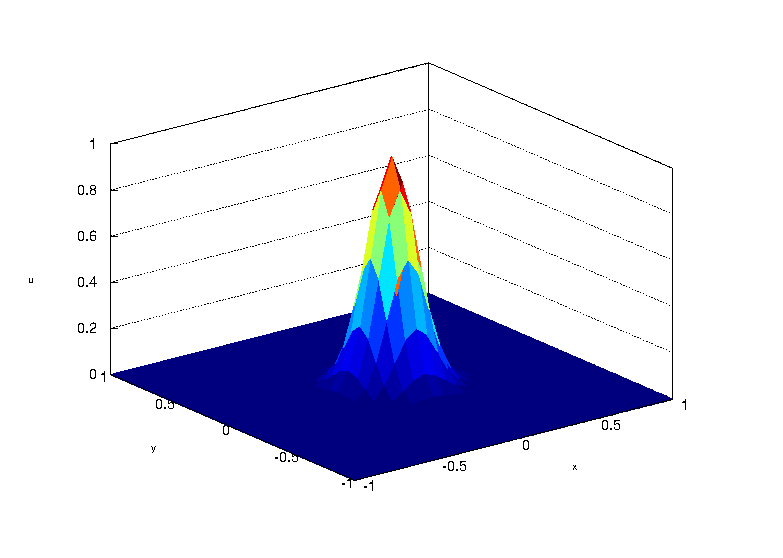
\includegraphics[width=1.0\textwidth]{photos/initialheat}
\end{center}
\end{column}
\begin{column}{0.5\textwidth}
approximate solution $u(t,x,y)$ at $t=0.02$ with $\Delta t=0.001$ 

\bigskip
\begin{center}
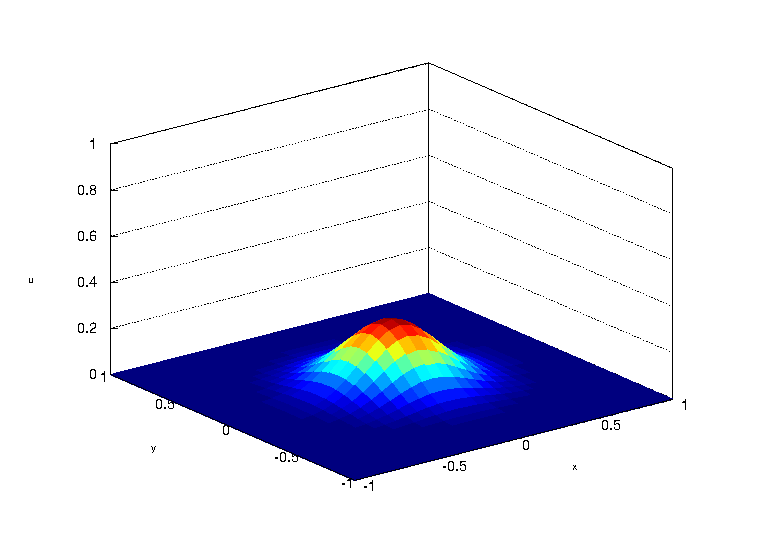
\includegraphics[width=1.0\textwidth]{photos/finalheat}
\end{center}
\end{column}
\end{columns}
\end{frame}


\begin{frame}{the look of instability}

\begin{itemize}
\item both figures are from solving $u_t = D(u_{xx} + u_{yy})$ on the same $50\times 50$ grid, at same final time and with same $D$, but with slightly different time steps
\end{itemize}

\bigskip
\begin{columns}
\begin{column}{0.5\textwidth}
\begin{center}
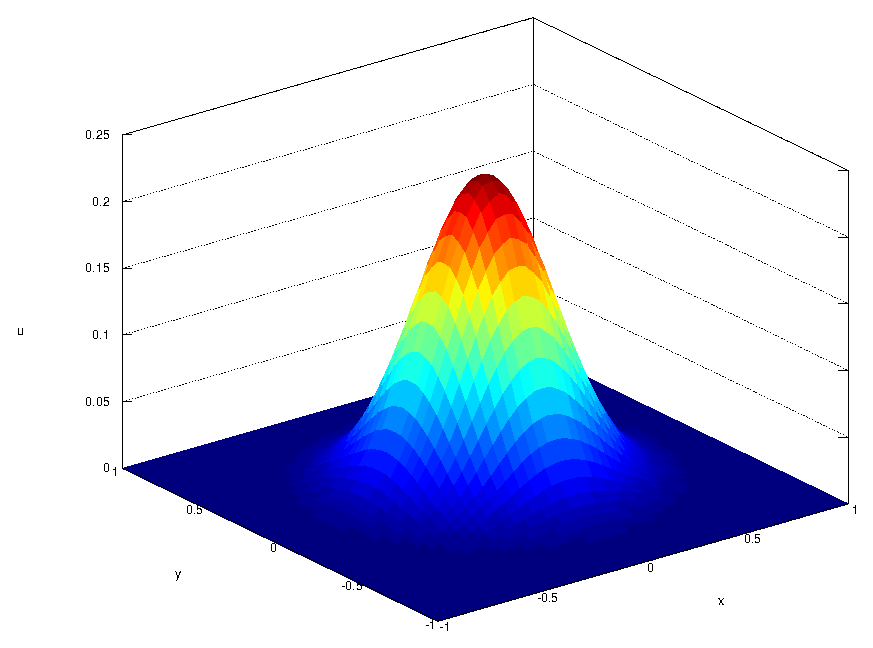
\includegraphics[width=1.0\textwidth]{photos/stability}
%$D=1,\Delta t = 0.00064286,\Delta x = \Delta y = 0.04$ so
  $$FIXME: see notes \frac{D\Delta t}{\Delta x^2}= 0.402$$
\end{center}
\end{column}
\begin{column}{0.5\textwidth}
\begin{center}
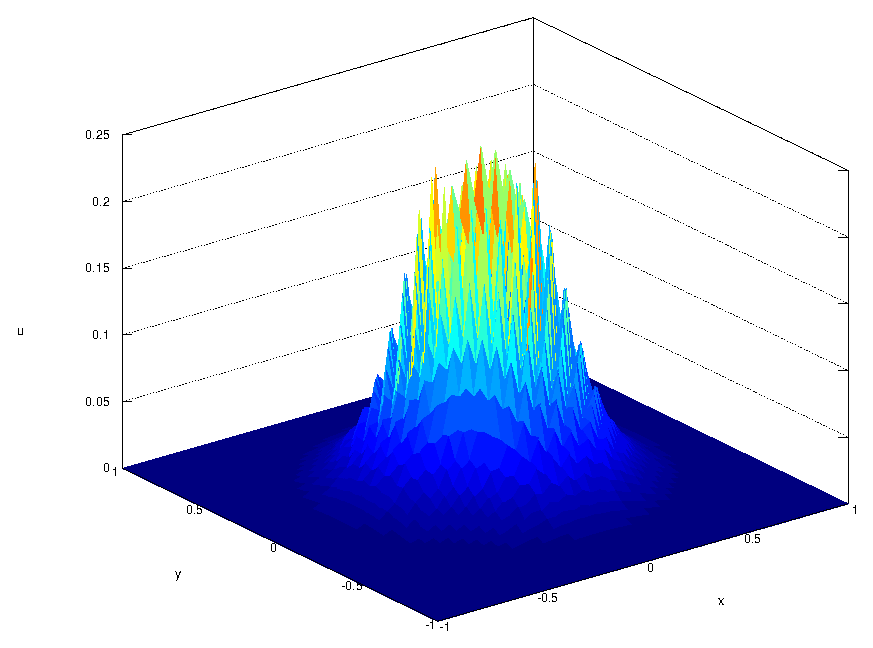
\includegraphics[width=1.0\textwidth]{photos/instability}
%$D=1,\Delta t = 0.001,\Delta x = \Delta y = 0.04$ so
  $$FIXME: see notes \frac{D\Delta t}{\Delta x^2}= 0.625$$
\end{center}
\end{column}
\end{columns}
\end{frame}


\begin{frame}{why unstable?}
\label{slide:maxprinc}

\begin{itemize}
\item the 1D first-order explicit scheme in the form 
	$$u_j^{n+1} = \nu u_{j+1}^n + (1 - 2 \nu) u_j^n + \nu u_{j-1}^n$$
gives new value $u_j^{n+1}$ as an \emph{average} of old values,
\item but it is only an average if the middle coefficient is positive:\footnote{recommended basic reference for finite differences, including stability: [Morton and Mayers, 2005]\nocite{MortonMayers}}
	$$1 - 2 \nu = 1 - 2 \frac{D\Delta t}{\Delta x^2} \ge 0$$
\item true averaging is always stable because averaged wiggles are smaller than the previous wiggles
\item ``positive coefficients'' is a \emph{sufficient} stability criterion
\item the same thing as a time-step restriction:
	$$\Delta t \le \frac{\Delta x^2}{2 D}$$
\end{itemize}
\end{frame}


\begin{frame}{\textsl{adaptive} implementation: guaranteed stability}

\minput{heatadapt}

\small
\begin{itemize}
\item same as \texttt{heat.m} except it gets the time step from:
	$$\frac{D\Delta t}{(\min\{\Delta x,\Delta y\})^2} \le \frac{1}{4}$$
\end{itemize}\end{frame}


\begin{frame}{alternative instability fix: implicitness}

\begin{columns}[T]
\begin{column}{0.7\textwidth}
\small
\begin{itemize}
\item explicit scheme is only ``conditionally stable'', but there are methods which are stable for \emph{any} positive time step $\Delta t$
\item the simplest such is \emph{first-order implicit} $\to$,
	$$\frac{u_j^{n+1} - u_j^n}{\Delta t} = D\,\frac{u_{j+1}^{n+1} - 2 u_j^{n+1} + u_{j-1}^{n+1}}{\Delta x^2}$$
\item another is \emph{Crank-Nicolson} $\to$; instead of $O(\Delta t,\Delta x^2)$ like first-order explicit and implicit, Crank-Nicolson is $O(\Delta t^2,\Delta x^2)$
\end{itemize}
\end{column}
\begin{column}{0.3\textwidth}
\includegraphics[width=1.2\textwidth]{pdffigs/impstencil}

\bigskip
\includegraphics[width=1.2\textwidth]{pdffigs/cnstencil}
\end{column}
\end{columns}

\begin{itemize}
\small
\item \emph{but} for implicit and Crank-Nicolson methods you have to solve systems of equations to take each step
\medskip

\item \scriptsize Donald Knuth has advice for ice sheet modelers: \begin{quote}
\emph{We should forget about small efficiencies, say about 97\% of the time: premature optimization is the root of all evil}.
\end{quote}
\end{itemize}
\end{frame}


\begin{frame}{variable diffusivity and time steps}

\begin{itemize}
  \item recall analogy \qquad (SIA) $\leftrightarrow$ (heat eqn)
  \item the SIA has a diffusivity $D$ which varies in time and space, so by analogy:
  		$$u_t = M + \Div \left(D(t,x,y) \grad \right)$$
  \item the explicit method is conditionally stable with the ``same'' stability condition \emph{if} we evaluate diffusivity $D(t,x,y)$ at \alert{staggered} grid points:
  \scriptsize
\begin{align*}
\Div \left(D(t,x,y) \grad u\right) &\approx \frac{D_{j+1/2,k}(u_{j+1,k} - u_{j,k}) - D_{j-1/2,k}(u_{j,k} - u_{j-1,k})}{\Delta x^2} \\
	&\qquad + \frac{D_{j,k+1/2}(u_{j,k+1} - u_{j,k}) - D_{j,k-1/2}(u_{j,k} - u_{j,k-1})}{\Delta y^2}
\end{align*}
\end{itemize}

\vspace{-0.15in}
\small
\begin{columns}
\begin{column}{0.55\textwidth}
in stencil at right:
\begin{itemize}
\item[] diamonds: $u$
\item[] triangles: $D$
\end{itemize}
\end{column}
\begin{column}{0.45\textwidth}
\begin{center}
\vspace{-0.15in}
\includegraphics[width=1.0\textwidth]{pdffigs/diffstencil}
\end{center}
\end{column}
\end{columns}
\end{frame}


\begin{frame}
  \frametitle{general diffusion equation code}

\minput{diffusion}

\small
\begin{itemize}
\item solves abstract diffusion equation $u_t = \Div \left(D(x,y)\, \grad u\right)$
\item user must supply diffusivity on staggered grid
\end{itemize}
\end{frame}


\subsection{exact solutions}

\begin{frame}{on exact solutions}

\begin{itemize}
\item I am not quite done with the (heat) $\leftrightarrow$ (SIA) analogy
\item \dots I also want to use it to address exact solutions and verification

\bigskip
\item the two senses of ``solution'':
  \begin{itemize}
  \small
  \item[$\circ$] a \emph{solution} $u(t,x,y)$ of the heat equation is a function of time and space for which $u_t = M + \Div (D\, \grad u)$ is true
  \item[$\circ$] a \emph{solution} of the heat equation is a \emph{prediction} of that model
  \normalsize
  \end{itemize}
\item exact solutions are exact predictions of the model, but not exact predictions about nature
\item if we can only \emph{approximately} find solutions of a model then knowing a few exact solutions can help test and maintain the quality of the actual code that does the approximation \dots this is \emph{verification} [Wesseling, 2001]\nocite{Wesseling}
\end{itemize}
\end{frame}


\begin{frame}{exact solutions of heat equation}

\begin{itemize}
\item \emph{many} solutions to the heat equation are known, but one is ``fundamental'' to the time-dependent equation, namely the Green's function
\end{itemize}

\begin{columns}[b]
\begin{column}{0.5\textwidth}
\begin{itemize}
\small
\item as time goes it changes shape by shrinking the output (vertical) axis and simultaneously lengthening the input (horizontal) axis
\item \dots \emph{but otherwise it is the same shape}, so it is self-similar
\item there are solutions of the SIA just like this
\normalsize
\end{itemize}
\end{column}
\begin{column}{0.5\textwidth}
\begin{center}
\includegraphics[width=1.0\textwidth]{pdffigs/heatscaling}

\emph{increasing time} \Large $\to$
\end{center}
\end{column}
\end{columns}
\end{frame}


\begin{frame}{finding the Green's function of the heat equation}

\begin{itemize}
\item the best-known way to find the Green's function of the heat equation is by Fourier transform, but we use a method which generalizes to the SIA
\item facts used to find it:
  \begin{itemize}
    \item[$\circ$] the Green's function starts at time $t=0$ with a \emph{delta function} at the origin $r=0$
    \item[$\circ$] the Green's function is angularly-symmetric:  $u$ is a function of the polar coordinate $r = \sqrt{x^2+y^2}$
    \item[$\circ$] calculus says: if $f=f(r)$ then $\grad^2 f = r^{-1} \left(r f'\right)'$
    \item[$\circ$] thus the heat equation in 2D, without additional heat sources, with constant diffusivity $D>0$, and for a function of $r$, is:
   $$u_t = D r^{-1} \left(r u_r\right)_r$$
  \end{itemize}
\item we use above facts to get Green's function by its ``similarity'' properties
\item \emph{but} we do not use the linearity of the heat equation
\end{itemize}
\end{frame}


\begin{frame}{finding a ``similarity'' solution of heat equation}
\label{slide:heatsim}

\small
\begin{itemize}
\item function $u(t,r)$ is replaced by function $\phi$ of one new variable $s$
\item input scaling: $s = t^{-\beta} r$
\item output scaling: $u = t^{-\alpha} \phi(s)$
\item chain rule says:
\begin{align*}
  u_t &= -\alpha t^{-\alpha-1} \phi - \beta t^{-\alpha-\beta-1} r \phi', \qquad u_r = t^{-\alpha-\beta} \phi', \qquad \text{etc.}
\end{align*}
\item so heat equation $u_t = D r^{-1} \left(r u_r\right)_r$ is replaced by:
	$$-\alpha \phi - \beta s \phi' = D s^{-1} t^{-2\beta+1} \left(\phi' + s \phi''\right)$$
\item choose $\boxed{\beta=1/2}$ so equation has no ``$t$'' and further simplify to
   $$-\frac{1}{2} \left[2 \alpha s \phi + s^2 \phi'\right] = D \left(s\, \phi'\right)'$$
\item choose $\boxed{\alpha = 1}$ so that quantity in square brackets simplifies to a derivative: $2 \alpha s \phi + s^2 \phi' = \left(s^2 \phi\right)'$
\end{itemize}
\end{frame}


\begin{frame}{finding a ``similarity'' solution of heat equation 2}

\small
\begin{itemize}
\item simplify and integrate, choose $C=0$, integrate again:
\begin{align*}
  - \frac{1}{2} s^2 \phi &= D\, s\,\phi' + C\\
  \phi' &= - \frac{s}{2D} \phi \\
  \phi(s) &= A e^{-s^2/(4D)}
\end{align*}
\item return to original variables, recalling $s = t^{-\beta} r$:
	$$u(t,r) = A\,t^{-1}\, e^{-r^2/(4Dt)} = A\,t^{-1}\, e^{-(x^2+y^2)/(4Dt)}$$
\item it is a spreading gaussian distribution
\item heat equation is linear so \emph{all} time-dependent solutions of the heat equation are convolutions with this solution \dots which is why it is \emph{fundamental}
\end{itemize}

\begin{center}
\animategraphics[autoplay,loop,height=2cm]{4}{anim/heatmelt}{0}{16}
\end{center}
\end{frame}


\begin{frame}{similarity solutions}

\begin{itemize}
\item \emph{conclusion from previous slides}: similarity variables for heat equation are
	$$s \stackrel{\text{\emph{input scaling}}}{\phantom{\Big|}=\phantom{\Big|}} t^{-\beta} x, \qquad u(t,x) \stackrel{\text{\emph{output scaling}}}{\phantom{\Big|}=\phantom{\Big|}} t^{-\alpha} \phi(s)$$
\item dimension dependence:
	\begin{tabular}{l|ccc}
	               & 1D & 2D & 3D \\ \hline
	input scaling ($t^{-\beta}$)   & $t^{-1/2}$ & $t^{-1/2}$ & $t^{-1/2}$ \\
	output scaling ($t^{-\alpha}$) & $t^{-1/2}$ & $t^{-1}$ & $t^{-3/2}$
	\end{tabular}
\end{itemize}
\begin{columns}
\begin{column}{0.6\textwidth}
\emph{historical note}:  In 1905 Einstein saw that the average distance traveled in time $t$ by particles in thermal motion goes like $\sqrt{t}$.  This is a microscopic explanation of the similarity variable $s = t^{-1/2}x$.
\end{column}
\begin{column}{0.4\textwidth}
\hfill \includegraphics[width=0.8\textwidth]{photos/brownian}
\end{column}
\end{columns}
\end{frame}


% Copyright 2009--2010  Ed Bueler

\section{shallow ice sheets}

\subsection{solving the SIA}

\begin{frame}{similarity solution to the SIA}

\begin{itemize}
\item jump forward to 1981 \dots breaking news: \quad P.~Halfar finds the fundamental solution of the SIA! \quad [Halfar, 1981; 1983]
\item when $n=3$, Halfar's 2D solution for Glen flow law has scalings
   $$H(t,r)=t^{-1/9} \phi(s), \qquad s = t^{-1/18} r$$
\item \dots therefore, if an ice sheet starts steep and it flows without additional accumulation then its thinning \emph{really} slows down as the shape flattens out
\end{itemize}

\medskip
\begin{center}
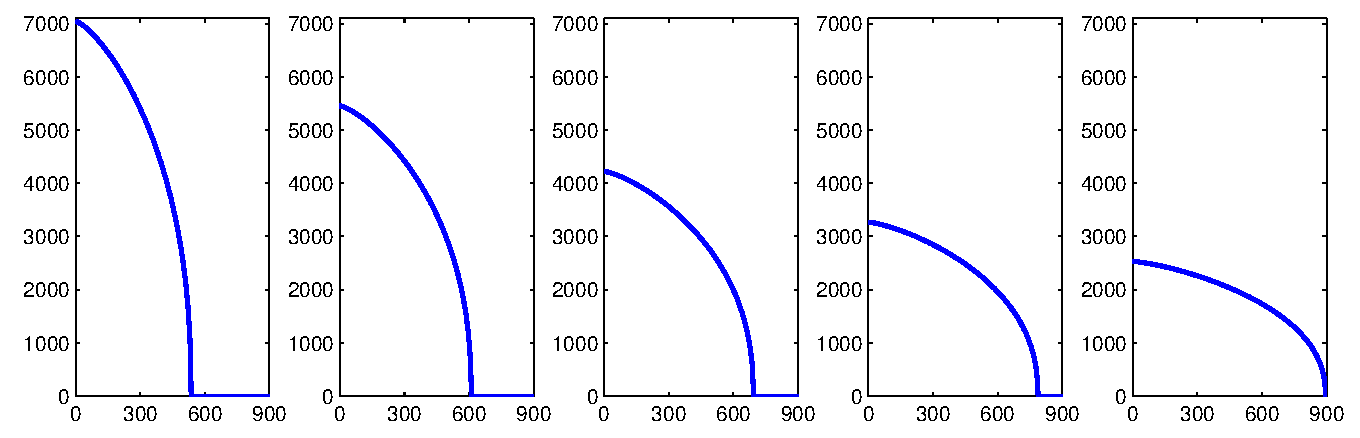
\includegraphics[width=0.95\textwidth]{pdffigs/siascaling}

\medskip
\scriptsize times 1, 10, 100, 1000, 10000 years
\end{center}
\end{frame}


\begin{frame}{similarity solution to the SIA 2}
\label{slide:plothalfar}

\animategraphics[autoplay,loop,height=7.0cm]{4}{anim/halfar}{0}{26}

\par
\scriptsize 
frames from $t=4$ months to $t = 10^6$ years, equal spaced in \emph{exponential} time
\end{frame}


\begin{frame}{similarity solution to the SIA 3}

\begin{itemize}
\item for $n=3$ the solution is:
  $$H(t,r) = H_0 \left(\frac{t_0}{t}\right)^{1/9} \left[1 - \left(\left(\frac{t_0}{t}\right)^{1/18} \frac{r}{R_0}\right)^{4/3}\right]^{3/7}$$
where
  $$t_0 = \frac{1}{18 \Gamma} \left(\frac{7}{4}\right)^3 \frac{R_0^4}{H_0^{7}}$$
and $H_0$, $R_0$ are central height and ice cap radius at $t=t_0$
\item you choose $H_0$ and $R_0$, and these determine the ``characteristic'' time $t_0$
\end{itemize}

\begin{center}
\tiny  more on this in [Nye, 2000] and [Bueler and others, 2005]
\end{center}
\end{frame}


\begin{frame}{finding Halfar solution}

\small
\emph{the method is the same as that which found the fundamental solution of the heat equation}:
\mode<presentation>{\scriptsize}
\begin{itemize}
\item allow scaling of the input and output:\qquad  $s = t^{-\beta} r$, \quad $H(t,r) = t^{-\alpha} \varphi(s)$
\item insert into $H_t = \Div \left(\Gamma H^{5} |\grad H|^{2} \grad H \right)$ \qquad\qquad ($\leftarrow$ \emph{$n=3$ case for simplicity})
\item to eliminate $t$ from the equation, choose $\boxed{7\alpha + 4\beta = 1}$; get
	$$-\alpha \phi - \beta s \varphi' = s^{-1} \left(\Gamma s \varphi^5 |\varphi'|^2\varphi'\right)'$$
\item to write as equality of derivatives, choose $\boxed{-\alpha + 2\beta=0}$:
	$$\left(-\beta s^2 \varphi\right)' = \left(\Gamma s \varphi^5 |\varphi'|^2\varphi'\right)'$$
\item integrate this and use finiteness of $\varphi(0)$, $\varphi'(0)$, and use $\varphi'(s)\le 0$, to get separable ODE
	$$\beta s = \Gamma \varphi^4 (-\varphi')^3$$
\item suppose $H(t_0,0)=H_0$ for some $t_0>0$ to find formula
	$$\varphi(s)^{7/3} = (t_0^\alpha H_0)^{7/3} - \frac{7}{4} \left(\frac{\beta}{\Gamma}\right)^{1/3} s^{4/3}$$
\item write as formula for $H(t,r)$, on previous slide, by solving boxed equations above to get $\alpha=1/9$, $\beta = 1/18$
\item margin location equation $\phi(t_0^{-\beta} R_0)=0$ gives formula for $t_0$ on previous slide
\mode<article>{
\item cases $n\ne 3$, isostatic bed shape, and $M\ne 0$ generalizations in [Bueler and others, 2005]
}
\end{itemize}
\end{frame}


\begin{frame}{evaluating Halfar solution}

\minput{halfar}

\begin{itemize}
\item it is easy to compute it, so \dots
\item \emph{please} use it to verify SIA codes, o.k.?
\end{itemize}
\end{frame}


\begin{frame}{is the Halfar solution \emph{good for any modeling}?}

\begin{itemize}
\item Nye and others [2000] compared the long-time consequences of different flow laws for the South Mars Polar Cap
\item they compared the long-time behavior of the corresponding \emph{Halfar solutions} for the different flow laws, with both $\text{CO}_2$ ice and $\text{H}_2\text{O}$ ice parameters
\item conclusions:
  \begin{quote}
  \dots none of the three possible [$\text{CO}_2$] flow laws will allow a 3000-m cap, the thickness suggested by stereogrammetry, to survive for $10^7$ years, indicating that the south polar ice cap is probably not composed of pure $\text{CO}_2$ ice \dots the south polar cap probably consists of water ice, with an unknown admixture of dust.
  \end{quote}
\item in 2008, NASA's Phoenix lander found water ice in the north polar cap on Mars
\end{itemize}
\end{frame}


\begin{frame}{on \textsl{degenerate} diffusivity}

\begin{itemize}
\item recall that the SIA is
\small
	$$H_t = M + \Div \left(D\, \grad h \right) \quad \text{where} \quad D = \Gamma H^{n+2} |\grad h|^{n-1}$$
\normalsize
\item ``degeneracy'' of $D$ happens in two ways:

\bigskip
\small
\begin{tabular}{l|c|c}
 & why $D\to 0$ & so what? \\ \hline
domes    & $\grad h \to 0$ & \begin{tabular}{c}
$H$ and $\grad h$ are continuous \\ but $\grad^2 h$ is singular
\end{tabular} \\ \hline
margins  & $H \to 0$       & \begin{tabular}{c}
$H$ is continuous \\ but $\grad h$ is singular
\end{tabular}
\end{tabular}
\normalsize
\bigskip

\item numerically, \emph{margins are worse than domes}
\item degenerate diffusion equations are free boundary problems
\item transformation $\eta = H^{(2n+2)/n}$ is known to help \dots for flat beds
\item as a practical matter, numerical solvers for the SIA must handle $u_t = M + \Div \left(D\, \grad u\right)$ for \emph{very} general diffusivity
\end{itemize}
\end{frame}


\begin{frame}
  \frametitle{computing diffusivity in SIA}

\begin{columns}
\begin{column}{0.6\textwidth}
\begin{itemize}
\item for numerical stability we want $D = \Gamma H^{n+2} |\grad h|^{n-1}$ on the staggered grid
\item various schemes proposed; stencil for Mahaffy [1976] scheme at right
\item all schemes involve
  \begin{itemize}
  \item[$\circ$] averaging $H$
  \item[$\circ$] differencing $h$
  \item[$\circ$] in a ``balanced'' way, for better accuracy,
  \end{itemize}
to put $D$ on the staggered grid
\end{itemize}
\end{column}

\begin{column}{0.4\textwidth}
  \includegraphics[width=1.0\textwidth]{photos/mahaffystencil}
\end{column}
\end{columns}
\end{frame}


\begin{frame}
  \frametitle{SIA implementation: flat bed case}

\minput{siaflat}
\end{frame}


\begin{frame}{the worst ice sheet}

\begin{itemize}
\item adaptive time-stepping works: \texttt{siaflat.m} takes short time steps when the driving stress $\rho g H |\grad h|$ is large, and then longer steps when it is ``easier''
\item for example, a worst-case ice sheet is \emph{thick} but with a \emph{very bumpy surface}
\item \texttt{roughice.m} generates initial ice sheet, which is thick and with a white-noise surface, then runs for 50 years
\item initial surface, final surface, and time-steps shown below
\end{itemize}

\begin{center}
\includegraphics[width=0.3\textwidth]{photos/roughinitial}  \includegraphics[width=0.3\textwidth]{photos/roughfinal} \includegraphics[width=0.38\textwidth]{photos/roughtimesteps}
\end{center}
\end{frame}


\subsection{is it right?}

\begin{frame}{verification of numerical ice flow codes}
\begin{itemize}
\item how do we make sure a numerical scheme \emph{and its implementation} are right?  some available \emph{techniques}
  \begin{enumerate}
  \item  don't make any mistakes
  \item  ``eyeball'' the results when you change the code \dots if it looks right it is right
  \item  from the beginning, build-in a comparison to an exact solution (= verification)
  \end{enumerate}
\end{itemize}
\end{frame}


\begin{frame}[fragile]
\frametitle{verifying our SIA code \texttt{siaflat.m}}

\begin{columns}
\begin{column}{0.6\textwidth}
\minputtiny{verifysia}
\end{column}

\begin{column}{0.4\textwidth}
\small
\begin{itemize}
\item this code calls \texttt{siaflat.m}
\item with initial condition which is a $t_1$ Halfar solution
\item numerical code runs to later time $t_2$ and the compares to Halfar at $t_2$
\end{itemize}

\bigskip
\scriptsize
map of thickness error from

\qquad \texttt{>> verifysia(160,3.0)}:

\includegraphics[width=1.0\textwidth]{photos/siaerror}
\end{column}
\end{columns}
\end{frame}


\begin{frame}[fragile]
\frametitle{verifying our SIA code 2}

\begin{columns}
\begin{column}{0.65\textwidth}
\small
\begin{verbatim}
>> verifysia(20,24.0);
errors for 20 x 20 grid:
average thickness error  = 22.335
maximum thickness error  = 227.275
>> verifysia(40,12.0);
errors for 40 x 40 grid:
average thickness error  = 9.519
maximum thickness error  = 241.040
>> verifysia(80,6.0);
errors for 80 x 80 grid:
average thickness error  = 2.937
maximum thickness error  = 159.442
>> verifysia(160,3.0);
errors for 160 x 160 grid:
average thickness error  = 0.988
maximum thickness error  = 103.456
>> verifysia(200,2.0);
errors for 200 x 200 grid:
average thickness error  = 0.827
maximum thickness error  = 94.561
\end{verbatim}
\normalsize
\end{column}

\begin{column}{0.35\textwidth}
\small
\emph{Trust but verify.}
\medskip

\tiny (Ronald Reagan)

\bigskip\bigskip\bigskip

\includegraphics[width=0.95\textwidth]{photos/eismintone}

\scriptsize \emph{figure 2 in [Huybrechts and others, 1996]}
\end{column}
\end{columns}
\end{frame}


\begin{frame}[fragile]
\frametitle{numerical mass conservation}

\begin{itemize}
\item in addition to measuring geometry errors, we might want a numerical code not to lose mass!
\item again, \emph{the Halfar solution is a perfect tool}
  \begin{itemize}
  \item[$\circ$] because the Halfar exact solution has exact (continuum) volume conservation
  \end{itemize}
\item add numerical volume calculation to \texttt{verifysia.m}:
\small
\begin{verbatim}
>> verifysia(20)
vol1       =  3.96112407720492e+15
...
vol2approx =  3.96112407720492e+15
voldiff = 1.50000000000000e+00
\end{verbatim}
\normalsize
\item huh?  how can it be that good?
  \begin{itemize}
  \item[$\circ$] the Mahaffy [1976] scheme has local numerical mass conservation
  \item[$\circ$] but what about the margin where $H\to 0$?
  \item[$\circ$] \texttt{siaflat.m} implements boundary condition \quad ``$H\ge 0$''
  \item[$\circ$] apparently this boundary condition produces global numerical mass conservation to rounding error!
  \end{itemize}
\end{itemize}
\end{frame}


\subsection{application}

\begin{frame}{application to the Antarctic ice sheet}
\small
\begin{itemize}
\item at Karthaus 2009, a computer project: modify \texttt{siaflat.m} to
  \begin{itemize}
  \small
  \item allow arbitrary bed elevation $b(x,y)$
  \item allow arbitrary mass balance $M(x,y)$
  \item apply a marine-margin condition
  \end{itemize}
and then simulate the Antarctic ice sheet
\item my solution: 
  \begin{itemize}
  \small
  \item add 8 lines to \texttt{siaflat.m} in total, creating \texttt{siageneral.m}
  \item use the SeaRISE 5km data set for present-day Antarctica (NetCDF)
  \item add a page or so of code for pre- and post-processing
  \item do 40 ka run starting with present-day geometry
  \end{itemize}
\end{itemize}

\vspace{-0.15in}
\begin{columns}
\begin{column}{0.5\textwidth}
\begin{center}
\scriptsize
initial (observed) surface elevation
\includegraphics[width=0.8\textwidth]{photos/antinitial}
\end{center}
\end{column}
\begin{column}{0.5\textwidth}
\begin{center}
\scriptsize
40 ka (modeled) surface elevation
\includegraphics[width=0.8\textwidth]{photos/antfinal}
\end{center}
\end{column}
\end{columns}
\end{frame}


\begin{frame}{application to the Antarctic ice sheet 2}

\begin{columns}
\begin{column}{0.6\textwidth}
\begin{itemize}
\item volume grows
  \begin{itemize}
  \item[$\circ$] levels out at about $33 \times 10^6\,\text{km}^3$
  \item[$\circ$] compare present-day observed volume of $25 \times 10^6\,\text{km}^3$
  \item[$\circ$] exponential time of about 15 ka,
  \item[$\circ$] but exponential time is \emph{much} longer if our model were thermocoupled, because of long advection time-scale  
  \end{itemize}
\end{itemize}
\end{column}
\begin{column}{0.45\textwidth}
\includegraphics[width=1.0\textwidth]{photos/antvol}
\end{column}
\end{columns}

\begin{itemize}
\item I used $A = 3\times 10^{-16}\,\text{Pa}^{-3}\,\text{a}^{-1}$ 
  \begin{itemize}
  \item[$\circ$] which is an ``enhancement factor'' of 3, \scriptsize relative to the EISMINT I [Huybrechts and others, 1996] value of $A=10^{-16}$ used earlier\small
  \end{itemize}
\item an enhancement factor of 24 would make the volume level out at about the present-day value
\item \emph{pop quiz}:  why is that not a good idea?
\end{itemize}
\end{frame}


\subsection{the most basic shallow assumption}

\begin{frame}{the most basic shallow assumption}

\begin{columns}

\begin{column}{0.6\textwidth}
\begin{itemize}
\item careful derivation of the SIA is next
\item makes ``shallowness assumptions''
\item the most basic is a limitation which applies to \emph{all} shallow ice theories\footnote{\tiny e.g.~SIA, SSA, Blatter-Pattyn, SIA+SSA hybrids, \dots} but not to the general Stokes theory:

\begin{center}
\emph{the surface and base of the ice are given by differentiable functions} $z=h(t,x,y)$ \emph{and} $z=b(t,x,y)$
\end{center}
\item the configurations at right, with overhang in surface, are not allowed
\end{itemize}
\end{column}

\begin{column}{0.4\textwidth}
\includegraphics[width=1.0\textwidth]{pdffigs/sshape}
\vspace{20mm}

\includegraphics[width=1.0\textwidth]{photos/Serac2}
% uploader was Eltouristo at fr.wikipedia
% Description "sérac sur le galcier blanc qui mène au dôme des écrins avril 2006"
\end{column}
\end{columns}
\end{frame}


\begin{frame}{kinematic and mass continuity equations}

\begin{itemize}
\item what does this ``most basic shallow assumption'' get you?
\item \emph{answer:} a map-plane mass continuity equation
\item consider these three equations:
  \begin{itemize}
  \item[$\circ$]  the surface kinematical equation
  \item[$\circ$]  the base kinematical equation
  \item[$\circ$]  the map-plane mass continuity equation
  \end{itemize}
\item all three equations are important for shallow ice sheets and shelves, but \emph{any two imply the third}
\item the key facts we need:
  \begin{itemize}
  \item[$\circ$]  the incompressibility of ice
    $$u_x + v_y + w_z = 0$$
  \item[$\circ$]  the Leibniz rule for differentiating integrals
  \scriptsize
    $$\frac{d}{dx}\left(\int_{g(x)}^{f(x)} h(x,y)\,dy\right) = f'(x) h(x,f(x)) - g'(x) h(x,g(x)) + \int_{g(x)}^{f(x)} h_x(x,y)\,dy$$
  \end{itemize}
\end{itemize}
\end{frame}


\begin{frame}{kinematic and mass continuity equations 2}

\begin{itemize}
\item let $a$ be the surface mass balance function ($a>0$ is accumulation)
\item let $s$ be the basal melt rate function ($s>0$ is basal melting)
\item define the map-plane flux of ice,
	$$\bq = \int_{b}^{h} (u,v)\,dz = (\bar u, \bar v)\,H$$
\item the three equations are:
\begin{empheq}[left=\text{surface kinematical}\quad,innerbox=\fbox]{equation}
h_t = a - u\big|_h h_x - v\big|_h h_y + w\big|_h  \label{surfkine}
\end{empheq}
\begin{empheq}[left=\text{base kinematical}\quad,innerbox=\fbox]{equation}
b_t = s - u\big|_b b_x - v\big|_b b_y + w\big|_b  \label{basekine}
\end{empheq}
\begin{empheq}[left=\text{mass continuity}\quad,innerbox=\fbox]{equation}
H_t = M - \Div \bq \, \text{ where } M=a-s \label{masscontinuity}
\end{empheq}
\end{itemize}
\end{frame}


\begin{frame}{kinematic and mass continuity equations 3}
\label{slide:twoimplythird}

\small
for example, here is a sketch of how to show \quad \eqref{surfkine} \,\&\, \eqref{basekine} $\implies$ \eqref{masscontinuity}:
\mode<presentation>{\scriptsize}
\begin{enumerate}
\item recalling $H=h-b$ and $M=a-s$, the difference of \eqref{surfkine} and \eqref{basekine} is
\begin{equation}
H_t = M - u\big|_h h_x - v\big|_h h_y + w\big|_h + u\big|_b b_x + v\big|_b b_y - w\big|_b \tag{*}
\end{equation}
\item incompressibility gives difference of surface and base values of $w$ by integration,
\begin{equation}
w_z = - (u_x + v_y) \quad \implies \quad w\big|_h - w\big|_b = - \int_b^h (u_x + v_y)\,d\zeta \notag
\end{equation}
which reduces (*) to: 
\begin{equation}
H_t = M - u\big|_h h_x - v\big|_h h_y + u\big|_b b_x + v\big|_b b_y - \int_b^h (u_x + v_y)\,d\zeta  \tag{**}
\end{equation}
\item on the other hand, the Leibniz rule on $\bq = \int_{b}^{h} (u,v)\,dz$ gives
	$$\Div \bq = u\big|_h h_x + v\big|_h h_y - u\big|_b b_x - v\big|_b b_y + \int_b^h (u_x+v_y)\,dz$$
\item \dots which reduces (**) to
	$$H_t = M - \Div \bq$$
\end{enumerate}
\end{frame}


\begin{frame}{kinematic and mass continuity equations 4}

\begin{itemize}
\item papers have lots of calculations like on the previous slide
\item usually mixed in with other arguments about shallowness
\item most ice sheet models use the mass continuity equation to describe change in ice sheet geometry,
\item \dots but they could instead use the surface kinematical equation
\item in using a stress balance in a shallow theory, all we need to do is get the horizontal velocity $(u,v)$, which gives $\bq$ and thus the mass continuity equation
\item for example, the derivation of the SIA from Stokes needs to only go far enough to find an expression for the horizontal velocity $(u,v)$
\end{itemize}
\end{frame}


\subsection{flowline Stokes}

\begin{frame}{Stokes equations in $x,z$ plane flow case}

\begin{itemize}
\item suppose all flow is in the (screen) $x,z$ plane
\item \dots so out-of-plane velocity is zero ($v=0$) and all quantities are constant in $y$ direction ($\partial/\partial y = 0$)
\item the symmetric strain rate tensor has many zeros
	$$D_{ij} = \frac{1}{2}\left(\frac{\partial u_i}{\partial x_j} + \frac{\partial u_j}{\partial x_i}\right) = \begin{pmatrix}
  	D_{11} & 0 & D_{13} \\
  	0 & 0 & 0 \\
  	D_{13} & 0 & D_{33} \\
  	\end{pmatrix}$$
\item incompressibility of ice in plane flow case says $D$ has trace zero:
	$$u_x + 0 + w_z = D_{11} + D_{33} = 0$$
\item \dots so $D_{33} = - D_{11}$ in this case
\end{itemize}
\end{frame}


\begin{frame}{Stokes equations in $x,z$ plane flow case 2}

\begin{itemize}
\item recall that the Cauchy stress tensor $\sigma_{ij}$, with its pressure part $p$ removed, is called ``deviatoric'':
	$$\tau_{ij} = \sigma_{ij} + p \delta_{ij} \qquad \text{where} \qquad p = -(1/3) (\sigma_{11} + \sigma_{22} + \sigma_{33})$$
\item the deviatoric stress tensor $\tau_{ij}$ is proportional to the tensor $D_{ij}$, in the isotropic (Glen law) case:
	$$D_{ij} = A(T) \tau^{n-1} \tau_{ij}$$
\item \dots where \quad $2 \tau^2 = 2 ({II}_\tau)^2 = \tau_{ij} \tau_{ij}$ \quad so \quad $\tau = \left(\tau_{11}^2 + \tau_{13}^2\right)^{1/2}$
\item so $\tau_{ij}$ is also symmetric, and has trace zero,
\item and $\tau_{ij}$ has only two nonzero entries $\tau_{11}$, $\tau_{13}$:
  	$$\begin{pmatrix}
  	\tau_{11} & 0 & \tau_{13} \\
  	0 & 0 & 0 \\
  	\tau_{13} & 0 & -\tau_{11} \\
  	\end{pmatrix}$$
\end{itemize}
\end{frame}


\begin{frame}{Stokes equations in $x,z$ plane flow case 3}

\begin{itemize}
\item in the 3D case: $n=3$, Glen, isothermal Stokes equations:
\begin{align*}
u_x + v_y + w_z &= 0 \\
0 &= \nabla \cdot \sigma + \rho \mathbf{g} \\
D_{ij} &= A \tau^2 \tau_{ij}
\end{align*}
\item $x,z$ plane flow case: from simplifications on previous slides, the isothermal Stokes equations say
\begin{empheq}[box=\fbox]{align}
u_x + w_z &= 0 \notag \\
p_x &= \tau_{11,x} + \tau_{13,z} \notag \\
p_z &= \tau_{13,x} - \tau_{11,z} - \rho g \label{Stokes} \\
u_x &= A \tau^2 \tau_{11} \notag \\
u_z + w _x &= 2 A \tau^2 \tau_{13} \notag
\end{empheq}
\item five scalar equations in five scalar unknowns ($u,w,p,\tau_{11},\tau_{13}$) but still fairly hard to solve \dots
\end{itemize}
\end{frame}


\begin{frame}{Stokes equations in $x,z$ plane flow case 4}

\begin{itemize}
\item previous equations apply within the ice fluid
\item \dots but \emph{boundary conditions are needed}
\item at the upper surface there is no stress from the air: $\sigma_{ij} n_j = 0$ where $\mathbf{n}$ is a normal vector to the surface
\item in plane flow case use $\mathbf{n} = (h_x,0,-1)$, which is gradient of $F(x,z)=h(x)-z$, which is constant on $z=h(x)$
\item get stress equations at surface:
\begin{align*}
\tau_{13} &= (\tau_{11} - p) h_x \\
p + \tau_{11} + \tau_{13} h_x &= 0
\end{align*}
\item we will only consider non-sliding SIA, so base boundary conditions are
   $$u=0 \quad \text{ and } \quad w=0$$
\end{itemize}
\end{frame}


\subsection{derivation of SIA}


\begin{frame}{scaling the variables}
\label{slide:siascalings}

\begin{itemize}
\item following Chapter 18 of [Fowler, 1997], \emph{Mathematical Models in the Applied Sciences}
  \begin{itemize}
    \scriptsize
    \item which does a much more general job than here: 3D case with conservation of energy, while we only do 2D isothermal case
    \item we also miss Andrew standing on a table and singing, too
    \normalsize
  \end{itemize}
\item consider ice sheet of typical depth $d$ and length $\ell$, and with velocity ($[u]$), deviatoric stress ($[\tau]$), and softness ($[A]$) scales
\item $\eps = d/\ell$ is the ``aspect ratio'' of the ice sheet
\item change to new starred variables using scales:\small
\begin{align*}
x &= \ell\, x^* &         u &= [u] u^* \\
z &= d\, z^*    &         w &= \eps [u] w^* \\
h &= d\, h^*    & \tau_{11} &= \eps [\tau] \tau_{11}^* \\
H &= d\, H^*    & \tau_{13} &= [\tau] \tau_{13}^* \\
A &= [A] A^*  & p - \rho g (h-z) &= \eps [\tau] p^*
\end{align*}
\normalsize
\end{itemize}
\end{frame}


\begin{frame}{scaling the variables 2}

\begin{itemize}
\item we will necessarily choose relations among the scales
\item the choice of such relations affects the outcome and is subject to ``scientific judgment'' (i.e.~controversy)
\item ``\dots the purpose is to attain `properly scaled' equations in which the largest dimensionless parameters are numerically of order one \dots'' [Fowler, 1997]
\item \emph{method}: we rewrite the Stokes equations and the boundary conditions in the newly (starred) variables, \emph{then} check that the scaling relations give reasonable values, \emph{then} remove terms to get a new, more-solvable model, the SIA
\item the scaling relations used here are:
\begin{align*}
\begin{matrix}
\text{balance of shear stress} \\
\text{and pressure gradient}
\end{matrix} && [\tau] &= \rho g d \eps \\
\text{balance of flow law scales} && \frac{[u]}{d} &= 2 [A] [\tau]^3
\end{align*}
\end{itemize}
\end{frame}


\begin{frame}{scaling the equations}

\small
\emph{example}:
\begin{itemize}
\item recall this equation from Stokes equations \eqref{Stokes}:
  $$p_x = \tau_{11,x} + \tau_{13,z}$$
\item replace all variables with their starred versions:
  $$\frac{\eps [\tau]}{\ell} p^*_{x^*}+ \frac{d \rho g}{\ell} h^*_{x^*} = \frac{\eps [\tau]}{\ell} \tau^*_{11,x^*} + \frac{[\tau]}{d}\tau^*_{13,z^*}$$
\item multiply by $\ell / (\eps [\tau])$:
  $$p^*_{x^*}+ \frac{d \rho g}{\eps [\tau]} h^*_{x^*} = \tau^*_{11,x^*} + \frac{\ell}{d \eps}\tau^*_{13,z^*}$$
\item use relation $[\tau] = \rho g d \eps$ and $\eps = d/\ell$:
  $$p^*_{x^*}+ \eps^{-2} h^*_{x^*} = \tau^*_{11,x^*} + \eps^{-2}\tau^*_{13,z^*}$$
\item re-arrange to taste and remove stars:
	$$h_x = \tau_{13,z} + \eps^2 \left(\tau_{11,x} - p_x\right)$$
\item \dots do this for each of the Stokes equations
\end{itemize}
%notes:
% if $f=[f]f^*$ and $x=[x]x^*$ for $f=f(x)$ then $f_x = \frac{[f]}{[x]} f^*_{x^*}$
% the scaling ``$p - \rho g (h-z) = \eps [\tau] p^*$'' implies $p=\eps [\tau]p^* + d \rho g (h^* - z^*)$
\end{frame}


\begin{frame}{scaling the equations 2}

\begin{itemize}
\item Stokes system now appears this way (\emph{stars are removed}):
\begin{align*}
u_x + w_z &= 0 \\
h_x &= \tau_{13,z} + \eps^2 \left(\tau_{11,x} - p_x\right) \\
p_z &= \tau_{13,x} - \tau_{11,z} \\
u_x &= \frac{1}{2} A \left(\eps^2 \tau_{11}^2 + \tau_{13}^2\right) \tau_{11} \\
u_z + \eps^2 w _x &= A \left(\eps^2 \tau_{11}^2 + \tau_{13}^2\right) \tau_{13}
\end{align*}
\item this is still full Stokes!
\item surface conditions are
\begin{align*}
\tau_{13} &= \eps^2 \left(\tau_{11} - p\right) h_x \\
p + \tau_{11} + \tau_{13} h_x &= 0
\end{align*}
\item base conditions are $u=0$ and $w=0$ as before
\end{itemize}
\end{frame}


\begin{frame}{checking the scales}

\begin{itemize}
\item the scale for vertical velocity is already chosen as $\eps [u]$
\item \dots and we now identify this scale with a typical value for accumulation: $[a] = \eps [u]$
\item thus we have chosen these scale relations:
  \begin{align*}
  \eps &= \frac{d}{\ell}           & [\tau] &= \rho g d \eps \\
  \frac{[u]}{d} &= 2 [A] [\tau]^3  &    [a] &= \eps [u]
  \end{align*}
\item to check their reasonableness, we will determine other scale factors in terms of $\ell$, $[a]$, and $[A]$, which are taken from observations:
  $$\ell = 3000\,\text{km},$$
  $$[a] = 0.1\,\text{m}\,\text{a}^{-1}$$
  $$[A] = 2 \times 10^{-16}\,\text{Pa}^{-3}\,\text{a}^{-1}$$
\end{itemize}
\end{frame}


\begin{frame}{checking the scales 2}

\begin{itemize}
\item solving for $d,\eps,[\tau],[u]$ gives
  \begin{align*}
  d &= \left(\frac{\ell^4 [a]}{2 [A] (\rho g)^3}\right)^{1/8} \approx 3600\,\text{m} \\
  \eps &= \frac{d}{\ell} \approx 10^{-3} \\
  [\tau] &= \rho g d \epsilon \approx 4 \times 10^4\, \text{Pa} = 0.4\,\text{bar}\\
  [u] &= 2 [A] d [\tau]^3 \approx 80\,\text{m}\,\text{a}^{-1}
  \end{align*}
\item these are all reasonable values for large ice sheets
\item it is reasonable to proceed to delete terms from the scaled equations to get the reduced (shallow) theory, the SIA
\item the actual measure of the quality of SIA is the comparison of its predictions to observations, when modeling various real ice sheets etc., \emph{not these scalings}
\end{itemize}
\end{frame}


\begin{frame}{finally get to the SIA}
\label{slide:siafinally}

\small
\begin{itemize}
\item setting $\eps=0$ in the scaled Stokes equations, get these equations (left column) and boundary conditions (right):
\begin{align*}
u_x + w_z &= 0                          & \tau_{13}\big|_h &\stackrel{\ast}{=} 0 \\
h_x &\stackrel{\ast}{=} \tau_{13,z}                      & p\big|_h + \tau_{11}\big|_h + \tau_{13}\big|_h h_x &= 0\\
p_z &= \tau_{13,x} - \tau_{11,z}        & & \\
u_x &= \frac{1}{2} A \tau_{13}^2 \tau_{11} & u\big|_b &\stackrel{\dagger}{=} 0 \\
u_z &\stackrel{\dagger}{=} A \tau_{13}^3 & w\big|_b &= 0
\end{align*}
\item combine the two marked ``$\ast$'', integrating vertically from surface $z=h$ to arbitrary elevation $z$, to get
	$$\tau_{13} = - (h - z) h_x$$
\item combine the two marked ``$\dagger$'', integrating vertically from base $z=b$ to arbitrary level $z$, and use the new expression for $\tau_{13}$, to get
\begin{align*}
u(z) &= A \int_b^z \tau_{13}^3\,d\zeta = - A (h_x)^3 \int_b^z (h - \zeta)^3\,d\zeta \\
     &= -\frac{A}{4} (h_x)^3 \left[H^4 - (h - z)^4\right]
\end{align*}

\end{itemize}
\end{frame}


\begin{frame}{finally get to the SIA 2}

\small
\begin{itemize}
\item remember I said that it suffices to find an expression for the horizontal velocity, in order to state the SIA?  \quad \emph{we are there!}
\item the previous slides have been in scaled quantities; now we recall the stars:
   $$u^* = -\frac{A^*}{4} (h^*_{x^*})^3 \left[(H^*)^4 - (h^* - z^*)^4\right]$$
\item and then unscale to find a dimensional expression for $u$, using $h^*_{x^*} = \eps^{-1} h_x$, and using scaling relations:
\begin{align*}
u &= [u] u^* = -\frac{[u] A}{4 [A]} \eps^{-3} (h_x)^3 d^{-4} \left[H^4 - (h - z)^4\right] \\
  &= - \left(\frac{[u]}{4 [A] \eps^3 d^4}\right) A (h_x)^3 \left[H^4 - (h - z)^4\right] \\
  &= - \left(\frac{2 [A] d (\rho g d \eps)^3}{4 [A] \eps^3 d^4}\right) A (h_x)^3 \left[H^4 - (h - z)^4\right] \\
  &= - \frac{1}{2} A (\rho g)^3 (h_x)^3 \left[H^4 - (h - z)^4\right]
\end{align*}
\end{itemize}
\end{frame}


\begin{frame}{finally get to the SIA 3}

\begin{itemize}
\item recall that the flux of ice is $q = \int_b^h u(z) \,dz$
\item so we integrate the expression for $u(z)$:
\begin{align*}
q &= -\frac{1}{2} A (\rho g)^3 (h_x)^3 \int_b^h \left[H^4 - (h - z)^4\right]\,dz \\
  &= -\frac{1}{2} A (\rho g)^3 (h_x)^3 \left[H^5 - \frac{1}{5}(H^5 - 0)\right] \\
  &= -\frac{2}{5} A (\rho g)^3 (h_x)^3 H^5
\end{align*}
\item the mass continuity equation now says:
\begin{align*}
H_t &= M - q_x = M + \left(\frac{2}{5} A (\rho g)^3 (h_x)^3 H^5\right)_x \tag{$\ast$}
\end{align*}
\item equation ($\ast$) matches equation \eqref{sia} in the plane flow case
\end{itemize}
\end{frame}


\begin{frame}{have I oversold diffusivity?} 

\begin{itemize}
\item I have asserted that the default model for ice sheets, the SIA, is a \emph{diffusion}
\item recall the analogy:

\bigskip
\begin{tabular}{ccc}
\emph{diffusion eqn} & $\leftrightarrow$ & \emph{SIA} \\ \hline
$u_t = \Div\left(D \grad u\right)$ & $\leftrightarrow$ & $h_t = M + \Div\left(D \grad h\right)$ \\
$D=D(x,y)$ & $\leftrightarrow$ & $D = \Gamma H^{n+2} |\grad h|^{n-1}$ \\
\end{tabular}

\bigskip
\item have I oversold this diffusivity analogy?
  \begin{itemize}
  \item[$\circ$] probably
  \item[$\circ$] \dots and I've acknowledged there are ``issues''
  \end{itemize}
\item but it turns out there is some robustness to my analogy
  \begin{itemize}
  \item[$\circ$] as follows on the next two slides
  \end{itemize}

\end{itemize}
\end{frame}


\begin{frame}{have I oversold diffusivity? 2}

\emph{DIFFUSIVE IDEA 1}: rough beds have the effect of \emph{reducing} diffusivity
\begin{itemize}
\item define the local bed topography by removing the local mean over some range $\lambda \approx 10$ km:
\small
   $$\tilde b(x,\xi) = b(x+\xi) - \fint_{-\lambda}^\lambda b(x+\xi)\,d\xi$$
\normalsize
\item define this strange average of the local bed:
\small
	$$\theta(x) = \left(\fint_{-\lambda}^\lambda \left(1 - \frac{\tilde b(x,\xi)}{H(x)}
                           \right)^{-(n+2)/n}\,d\xi\right)^{-1/n}$$
\normalsize
\item using a multiple-scales analysis, Schoof [2003] says you will get closer to solving the Stokes equations by making these two modifications of the SIA:
  \begin{itemize}
  \item[$\circ$] smooth the bed, \qquad \tiny \emph{(modelers want to do that anyway)} \small
  \item[$\circ$] but don't lose track of the smoothed-away local bed roughness; use it to reduce the diffusivity:
  \small
  		$$D_{\text{new}} = \theta D \qquad \text{where } 0 \le \theta \le 1$$
  \end{itemize}
\end{itemize}
\end{frame}


\begin{frame}{have I oversold diffusivity? 3}

\emph{DIFFUSIVE IDEA 2}: the large-scale effect of sliding in ice streams (\emph{addressed in next section}), is diffusive
\begin{itemize}
\item suppose that, for an ice stream modeled by the SSA equation
   $$\left(2 A^{-1/n} H |u_x|^{1/n - 1} u_x \right)_x - C|u|^{m-1}u = \rho g H h_x$$
we assume that the basal resistance term balances the driving stress:
   $$- C|u|^{m-1}u = \rho g H h_x$$
\item then the ice stream geometry evolves by a diffusion,
	$$h_t = M + \Div\left(D\,\grad h\right) \qquad \text{where } D = C' H^{(1/m)+1}|\grad h|^{(1/m)-1}$$
\item this ``outer problem'' is part of a matched asymptotic expansion that \emph{does a good job of tracking the grounding line in a marine ice sheet} [Schoof, 2007]
\end{itemize}
\end{frame}


% Copyright 2009--2010  Ed Bueler

\section{shelves and streams}

\subsection{shallow shelf approximation (SSA)}

\begin{frame}{the shallow shelf approximation (SSA) stress balance}
  
is a model which applies well to large ice shelves
\begin{itemize}
\item \dots for parts away from grounding lines
\item \dots and away from calving fronts
\end{itemize}

\mode<presentation>{
\begin{center}
  \includegraphics[width=0.7\textwidth]{photos/iceshelfedge}

\tiny edge of Ekstr\"om ice shelf, photo Hans Grobe, Polarstern expedition ANT-XX/2
\end{center}
}
\end{frame}


\begin{frame}{SSA stress balance 2}

\begin{columns}
\begin{column}{0.55\textwidth}
SSA also applies reasonably well to ice streams
\begin{itemize}
\item \dots with modest bed topography
\item \dots and weak bed strength
\end{itemize}
\end{column}

\begin{column}{0.45\textwidth}
%\includegraphics[width=1.0\textwidth]{photos/palmer_land}
%\tiny Palmer Land, Antarctica, photo 131 (Post \& LaChapelle 2000)\cite{PostLaChapelle}
  \includegraphics[width=1.0\textwidth]{photos/NEgreenlandJoughin}
\end{column}
\end{columns}

\bigskip\bigskip
\small
\emph{comment}:  energy conservation issues---both ice temperature and basal melt rate---are a major part of ice stream flow modeling [Raymond, 2000]\nocite{Raymondenergy}, \emph{but they are not addressed in these lectures}
\end{frame}


\begin{frame}{what is, \emph{and is not}, an ice stream?}

\begin{columns}
\begin{column}{0.6\textwidth}
\begin{itemize}
\item ice streams have fast flow ($50$ to $>1000 \,\text{m}\,\text{a}^{-1}$) by sliding, with
  \small
  \begin{itemize}
  \item[$\circ$] low bed resistance and
  \item[$\circ$] a critical role of \emph{liquid water} at bed [Clarke, 2005]\nocite{Clarke05}
  \end{itemize}
  \normalsize
\item ``outlet glaciers'' may have the same properties, but they have substantial vertical shear and proportionally less sliding
\item \emph{and} they have lower aspect ratio than ``true'' ice streams
\item \emph{and} some outlet glaciers are really fast, e.g.~Jakobshavn Isbrae
\item thus: \emph{few simplifying assumptions are possible for outlet glaciers}
\item not clear you should use SSA for outlet glaciers
\end{itemize}
\end{column}

\begin{column}{0.4\textwidth}
\mode<presentation>{
\includegraphics[width=1.0\textwidth]{photos/streamisbrae}

\bigskip
\scriptsize 
Cross sections of Jakobshavns Isbrae (\textbf{a}) and
Whillans Ice Stream (\textbf{b}).  Plotted
without vertical exaggeration in order to better illustrate
the difference between the two types.  (\tiny Figure 1 in [Truffer and Echelmeyer, 2003]\nocite{TrufferEchelmeyer})
}
\end{column}
\end{columns}
\end{frame}


\begin{frame}{stream-to-shelf flow line: notation again}
\begin{center}
  \includegraphics[width=0.96\textwidth]{photos/flowline}

\bigskip
\tiny \emph{figure modified from} [Schoof, 2007]\nocite{SchoofMarine1}
\end{center}
\end{frame}


\begin{frame}{the SSA equation}

\begin{itemize}
\item we will only work in plane flow case
\item we will numerically solve only the stress balance equation which determines the velocity in an ice shelf or ice stream:
\begin{empheq}[box=\fbox]{equation}
  \left({\color{blue}2 A^{-1/n} H |u_x|^{1/n - 1} u_x}\right)_x - C|u|^{m-1}u - \rho g H h_x = 0 \label{ssa}
\end{empheq}
  \begin{itemize}
  \scriptsize
  \item[$\circ$] derived originally by Morland [1987]\nocite{Morland}, MacAyeal [1989]\nocite{MacAyeal}
  \item[$\circ$] references: Weis and others [1999]\nocite{WeisGreveHutter}, Schoof [2006; 2007]\nocite{SchoofStream,SchoofMarine1}
  \normalsize
  \end{itemize}
\item the {\color{blue} blue term} inside parentheses is the vertically-integrated ``longitudinal'' or ``membrane'' stress

%\item two horizontal dimension ($x$ and $y$) version of this equation is significantly harder to solve numerically (Goldberg et al. 2009\cite{Goldbergetal2009})
\item \emph{how to solve this equation numerically}?
\item \emph{how to think about it}?
\end{itemize}
\end{frame}


\begin{frame}{the full monty, with a grounding line}
\label{slide:streamtoshelf}

\small
here is a full flow line context:
\begin{align*}
  u(0) = (\text{given}) \\
  \left.\begin{array}{r}
  \boxed{\left(2 A^{-1/n} H |u_x|^{1/n - 1} u_x\right)_x - C|u|^{m-1}u - \rho g H h_x = 0} \\
  H_t = M - (uH)_x \\
  \rho H \ge \rho_w (-b) \\
  h = H + b
  \end{array}\right\}& \text{ on } 0 < x < x_g \\
  h,u,u_x \text{ continuous at }& x=x_g \\
  \left.\begin{array}{r}
  \boxed{\left(2 A^{-1/n} H |u_x|^{1/n - 1} u_x\right)_x - \rho g (1-\rho/\rho_w) H H_x = 0} \\
  H_t = M - (uH)_x \\
  \rho H < \rho_w (-b)
  \end{array}\right\}& \text{ on } x_g < x < x_c \\
  \left.\begin{array}{r}
  2 A^{-1/n} H |u_x|^{1/n - 1} u_x - \frac{1}{2}\rho (1-\rho/\rho_w) g H^2 = 0 \\
  (\text{a condition describing movement of } x_c)
  \end{array}\right\}& \text{ at } x = x_c
\end{align*}
\small
\begin{itemize}
\item this is the default model in the Marine Ice Sheet Model Intercomparison Project [MISMIP; Schoof and others, 2008]\nocite{MISMIPwebpage}
\item \emph{effectively an open problem}:  what is best numerical treatment of grounding line movement in above model?
\end{itemize}
\end{frame}


\subsection{flow-line ice shelf}

\begin{frame}{exact thickness and velocity for steady ice shelf}


\begin{itemize}
\item we need a more limited goal!
\item \emph{first goal}:  solve the steady state ice shelf in the isothermal, plane flow, and Glen law case
\item for this nice situation, there is a nice result: the thickness and velocity in the ice shelf can be completely determined\footnote{e.g.~[van der Veen, 1985]\nocite{vanderVeen85}} from:
  \begin{enumerate}
  \item ice thickness $H_g$ at the grounding line,
  \item ice velocity $u_g$ at the grounding line,
  \item an integrable (e.g.~constant) surface balance $M(x)$
  \end{enumerate}
\item we do this by-hand on the next slide
\item we will use the by-hand result to:
  \begin{itemize}
  \item[$\circ$] understand the SSA, and
  \item[$\circ$] verify a numerical code
  \end{itemize}
\end{itemize}
\end{frame}


\begin{frame}{exact thickness and velocity for steady ice shelf 2}

\small
  \begin{enumerate}
  \item using flotation criterion $h = (1-\rho/\rho_w) H$, and because of no bed resistance, equation \eqref{ssa} says ``derivative of something $=0$'':
\begin{equation}
  \left(2 A^{-1/n} H |u_x|^{1/n - 1} u_x\right)_x - \left(\frac{1}{2} \rho g (1-\rho/\rho_w) H^2\right)_x = 0  \label{derivequalszero}
\end{equation}
  \item use the calving-front condition to integrate \eqref{derivequalszero}:
\begin{equation}
2 A^{-1/n} H |u_x|^{1/n - 1} u_x - \frac{1}{2} \rho g (1-\rho/\rho_w) H^2 = 0  \label{shelfsteadyu}
\end{equation}
  \item the steady  ($H_t=0$) mass continuity equation can be integrated; here $M=M_0=$constant but some other $M(x)$ are allowed:
\begin{equation}
uH = M_0(x-x_g) + u_g H_g,  \label{shelfsteadyflux}
\end{equation}
  \item multiply \eqref{shelfsteadyu} by $u/H$, replace $uH$ from \eqref{shelfsteadyflux}, assume positive strain rate ($u_x>0$), compute $n$th power
  \item get $u^n u_x = C_s \left(M_0(x-x_g) + u_g H_g\right)^n$, where $C_s$ is known
  \item integrate the last result to find $u(x)$, then return to \eqref{shelfsteadyflux} to find $H(x)$:
\begin{gather*}
u(x)^{n+1} = u_g^{n+1} + \frac{C_s}{M_0} \left[\left(M_0(x-x_g) + u_g H_g\right)^{n+1} - (u_g H_g)^{n+1}\right], \\
H(x) = \frac{M_0(x-x_g) + u_g H_g}{u(x)}
\end{gather*}
  \end{enumerate}
\end{frame}


\begin{frame}{exact thickness and velocity for steady ice shelf 3}

\small
\begin{itemize}
\item Matlab/Octave code \texttt{exactshelf.m} uses shelf length $L=200$ km, and $H_g=500$, $u_g = 50\,\text{m}\,\text{a}^{-1}$
\item computes this shelf geometry and velocity:
  \begin{center}
  \includegraphics[width=0.7\textwidth]{photos/shelfthk}

  \smallskip
  \includegraphics[width=0.7\textwidth]{photos/shelfvel}
  \end{center}
\end{itemize}
\end{frame}


\subsection{numerical solution}


\begin{frame}{numerically solving the SSA}

\begin{itemize}
\item the stress balance is a two-point boundary value problem (BVP) for the velocity $u(x)$:
\small
\begin{gather*}
\left(2 A^{-1/n} H |u_x|^{1/n - 1} u_x\right)_x - C|u|^{m-1}u - \rho g H h_x = 0, \\
\begin{matrix}
\text{\emph{left b.c.}:} & u(x_g) = u_g, \\
\text{\emph{right b.c.}:} & 2 A^{-1/n} H |u_x|^{1/n - 1} u_x - \frac{1}{2}\rho (1-\rho/\rho_w) g H^2 = 0 \text{ at } x = x_c
\end{matrix}
\end{gather*}
\normalsize
\item here we will prescribe the ice geometry, thus both the thickness $H(x)$ and the driving stress $\rho g H h_x$, and we will find the velocity $u(x)$
\item I'll describe the numerical method for a ice shelf \emph{or} ice stream
\item \dots but then I'll give a code \emph{only} for an ice shelf, so $C=0$ and $h=(1-\rho/\rho_w)H$
\end{itemize}
\end{frame}


\begin{frame}{numerically solving the SSA stress balance 2}

\begin{itemize}
\item like most such nonlinear equations, iteration is needed to solve this one
\item red term $\bar \nu = {\color{red} A^{-1/n} |u_x|^{1/n-1}}$ is the ``effective viscosity'':
   $$\left(2 {\color{red} A^{-1/n} |u_x|^{1/n-1}} H u_x\right)_x - C |u|^{m-1} u - \rho g H h_x = 0$$
\item let
   $$W(u_x) = 2 \bar \nu H = 2 A^{-1/n} |u_x|^{1/n-1} H$$
\item \emph{idea}: use old effective viscosity to get new velocity solution, and repeat until the solution is not changing too much and/or the differential equation is nearly-satisfied
\item \emph{idea as algorithm}: from $u^{(k-1)}$, find next values $u^{(k)}$ by solving the \emph{linear} problem
   $$\left(W(u^{(k-1)}_x) u^{(k)}_x\right)_x - C |u^{(k-1)}|^{m-1} u^{(k)} - \rho g H h_x = 0$$
\end{itemize}
\end{frame}


\begin{frame}{numerically solving the SSA stress balance 3}

where do you get an initial guess $u^{(0)}(x)$ for the velocity?
\medskip

\begin{itemize}
\item \emph{for floating ice}, a velocity comes from assuming a uniform strain rate:
   $$u^{(0)} = \gamma (x-x_g) + u_g$$
  \begin{itemize}
  \item[$\circ$]  for example: $\gamma$ is the value of $u_x$ found from the calving front stress imbalance and $u_g$ is the known velocity at the grounding line
  \end{itemize}
\item \emph{for grounded ice}, a velocity comes from assuming the ice is held by basal resistance only:
   $$u^{(0)} = \left(-C^{-1} \rho g H h_x\right)^{1/m}$$
\end{itemize}
\end{frame}


\begin{frame}{solving the ``inner'' linear problem}
\begin{itemize}
\item reset $x$ interval to be $0 < x < L$, instead of $x_g < x < x_c$
\item abstract the problem to a linear BVP:
   $$\left(W(x)\, u_x\right)_x - \alpha(x)\, u = \beta(x)$$
with boundary conditions
   $$u(0) = V, \qquad  u_x(L) = \gamma$$
\item $W(x)$, $\alpha(x)$, $\beta(x)$ are all known functions in this abstract problem
\item for the nonlinear SSA equation, both $W(x)$ and $\alpha(x)$ will come from the previous iteration
\item $W(x)$ is needed on the staggered grid, for $O(\Delta x^2)$ accuracy, as with time-dependent diffusion problem earlier
\item $\alpha(x),\beta(x)$ are needed on regular grid
\end{itemize}
\end{frame}


\begin{frame}{solving the ``inner'' linear problem 2}

\begin{itemize}
\item indices $j=1,2,\dots,J+1$
\item equal-spaced grid $x_1,x_2,\dots,x_{J+1}$, where $x_1 = 0$ and $x_{J+1} = L$
\item an approximation of the abstracted problem is:
$$\frac{W_{j+1/2} (u_{j+1} - u_j) - W_{j-1/2} (u_{j} - u_{j-1})}{\Delta x^2} - \alpha_j u_j \stackrel{\ast}{=} \beta_j$$
\item $u_1 = V$ given
\item for right-hand boundary condition ``$u_x(L)=\gamma$'':
  \begin{itemize}
  \item[$\circ$] introduce notional point $x_{J+2}$
  \item[$\circ$]
    $$\frac{u_{J+2} - u_J}{2 \Delta x} = \gamma$$
  \item[$\circ$] using equation $\ast$ in $j=J+1$ case, eliminate $u_{J+2}$ variable ``by-hand'' [Morton and Mayers, 2005]\nocite{MortonMayers}
  \end{itemize}
\end{itemize}
\end{frame}


\begin{frame}{solving the ``inner'' linear problem 3}

\scriptsize
\begin{itemize}
\item so abstract linear system has matrix-vector form `` $A \mathbf{x} = \mathbf{b}$ '':
$$
\begin{bmatrix}
1 &  &  &  &  \\
W_{3/2} & A_{22} & W_{5/2} &  &  \\
 & W_{5/2} & A_{33} &  &  \\
 &  & \ddots & \ddots &  \\
 &  & W_{J-1/2} & A_{JJ} & W_{J+1/2} \\
 &  &  & A_{J+1,J} & A_{J+1,J+1} \\
\end{bmatrix}\,
\begin{bmatrix}
u_1 \\ u_2 \\ u_3 \\ \vdots \\ u_J \\ u_{J+1}
\end{bmatrix}
=
\begin{bmatrix}
V \\ \beta_2 \Delta x^2 \\ \beta_3 \Delta x^2 \\ \vdots \\ \beta_J \Delta x^2 \\ b_{J+1}
\end{bmatrix}
$$
\item with diagonal entries  ($j=2,3,\dots,J$)
$$A_{jj} = -(W_{j-1/2}+W_{j+1/2}+\alpha_j \Delta x^2)$$
\item with special cases in last equation:
$$A_{J+1,J} = W_{J+1/2}+W_{J+3/2}$$
$$A_{J+1,J+1} = -(W_{J+1/2}+W_{J+3/2}+\alpha_{J+1}\Delta x^2)$$
$$b_{J+1} = -2 \gamma \Delta x W_{J+3/2} + \beta_{J+1} \Delta x^2$$
\item this is a \emph{tridiagonal} system
\end{itemize}
\end{frame}


\begin{frame}{solving the ``inner'' linear problem 4}
\label{slide:flowlinecode}

\minput{flowline}
\end{frame}


\begin{frame}{solving the ``inner'' linear problem 5}

\begin{itemize}
\item before proceeding to solve nonlinear SSA problem, we can test the ``abstracted'' code \texttt{flowline.m}
\item \dots by ``manufacturing'' solutions as in code \texttt{testflowline.m} \quad \scriptsize (not shown) \normalsize
\item \emph{results}: \quad works pretty well! converges at optimal rate $O(\Delta x^2)$
\end{itemize}

\begin{center}
  \includegraphics[width=0.65\textwidth]{photos/convanalysis}
\end{center}
\end{frame}


\begin{frame}{numerical solution to SSA}

\minputtiny{ssaflowline}
\end{frame}


\begin{frame}{\emph{numerical} thickness and velocity for steady ice shelf}

\begin{itemize}
\item first: let's numerically solve the problem for which we know exact answer
\item here use very coarse 10 km grid
\end{itemize}

\begin{center}
  \includegraphics[width=0.7\textwidth]{photos/shelfnumsoln}
\end{center}
\end{frame}


\begin{frame}[fragile]
  \frametitle{did we make any mistakes?}

\begin{itemize}
\item this does convergence analysis of \mname{ssaflowline.m}:

\scriptsize
\begin{verbatim}
J = [50 100 200 400 800 1600 3200];   dxkm = 200.0 ./ J;              
for j=1:length(J)
  [av,maxerr(j)] = testshelf(J(j));   % calls ssaflowline.m
end
loglog(dxkm,maxerr,'0-','markersize',16)
\end{verbatim}
\normalsize
\item goal is to see velocity error shrink by rate built-into our finite differences, namely at nearly the optimal rate $O(\Delta x^2)$
\item by this standard, we likely made no mistakes!
\end{itemize}

\begin{center}
  \includegraphics[width=0.55\textwidth]{photos/shelfconv}
\end{center}
\end{frame}


\begin{frame}{realistic ice shelf modeling}

\small
\begin{itemize}
\item flow lines (1D) are never very realistic \dots
\item ``diagnostic'' (= fixed geometry) ice shelf modeling in two horizontal variables (2D) has been quite successful
\item solve an \emph{elliptic} PDE boundary value problem
\item velocity measurements are available for validation
  \begin{itemize}
  \scriptsize
  \item[$\circ$] Ross ice shelf example based on [RIGGS; Bentley, 1974]\nocite{RIGGS1} data below: model (\alert{red} arrows) vs observations (\textbf{black} arrows)
  \item[$\circ$] this is PISM but many models can do it [MacAyeal and others, 1996]\nocite{MacAyealetal}
  \item[$\circ$] something of a mystery why regular grid methods do well!
  \small
  \end{itemize}
\end{itemize}

\begin{center}
  \includegraphics[width=0.6\textwidth]{photos/PISM_ross_speeds}
\end{center}
\end{frame}


\subsection{scaling up}

\begin{frame}{numerical solution of SSA: a summary}

\begin{itemize}
\item SSA and Blatter [1995]\nocite{Blatter} stress balance equations each
   \begin{itemize}
   \item[$\circ$]  determine horizontal velocity from geometry and b.c.s
   \item[$\circ$]  are nonlinear problems: require iterative linearization
   \item[$\circ$]  each ``inner'' linear problem has a sparse pattern
      \begin{itemize}
      \item[$\ast$] tridiagonal in SSA flow-line (1D) case here
      \item[$\ast$] much less structured in SSA 2D, Blatter 2D, and Blatter 3D cases
      \end{itemize}
   \end{itemize}
\item the Stokes stress balance is much harder because incompressibility must be handled explicitly
\item a wise numerical modeler would give the sparse linear problem to a numerical linear algebra software package:
  \begin{itemize}
  \item[$\circ$]  \Matlab/\Octave, \emph{LAPACK}, \emph{PETSc}, \emph{Trilinos}, \dots
  \item[$\circ$]  generally: modularize your code and \emph{test the parts separately}!
  \end{itemize}
\item \emph{comment} on mass continuity:  
  \begin{itemize}
  \item[$\circ$]  the mass continuity PDE ``$H_t = M - \Div\left(\bar \bu H\right)$'' is \emph{not} very diffusive if the source of $\bar \bu$ is SSA or Blatter,
  \item[$\circ$]  and there is \emph{not much theory} to guide how to solve such a generic transport problem
  \end{itemize}
\end{itemize}
\end{frame}


\begin{frame}{scaling-up the numerical solution of stress balances}

\begin{itemize}
\item all stress balance equations used for ice flow modeling are nonlinear equations for velocity $\bu$ in the form
	$$\bbF(\bu) = 0$$
\vspace{-0.1in}
\item the ``residual'' $\bbF$ involves various partial derivatives, nonlinear operations, and additional fields (e.g.~thickness)
\item SSA and Blatter stress balance equations can be written in form
	 $$\bA(\bu)\,\bu = \bg$$
\vspace{-0.15in}
  \begin{itemize}
  \item[$\circ$]  where $\bA$ is a nonlinear function of $\bu$,
  \item[$\circ$]  and $\bA(\bu)$ acts linearly on $\bu$
  \end{itemize}
\item we have already treated the SSA in the second way
\item both forms are nonlinear, elliptic PDEs
\item Newton [1669] knew a way of solving nonlinear equations!
\end{itemize}
\end{frame}


\begin{frame}{scaling-up the numerical solution of stress balances 2}

\begin{itemize}
\item the iteration scheme we have used for SSA is ``Picard'':
	$$\bA(\bu^{(k-1)})\,\bu^{(k)} = \bg$$
\vspace{-0.2in}
  \begin{itemize}
  \item[$\circ$] this iteration converges linearly, if it converges:  $\|\bu^{(k+1)} - \bu^{(k)}\| \le \gamma \|\bu^{(k)} - \bu^{(k-1)}\|$, where $0<\gamma<1$
  \item[$\circ$] it can be robust, but it is not fast
  \end{itemize}	
\item Newton's method (e.g.~[Press and others, 1992])\nocite{Pressetal} also solves $\bbF(\bu) = 0$ iteratively, but by linearization:
\begin{gather*}
J(\bu^{(k-1)})\,\bw = - \bbF(\bu^{(k-1)}), \\
\bu^{(k)} = \bu^{(k-1)} + \bw
\end{gather*}
\vspace{-0.1in}
where
   $$J(\bu)_{ij} = \frac{\partial \bbF(\bu)_i}{\partial \bu_j} \qquad \text{is the \emph{Jacobian} of } \bbF$$
\vspace{-0.1in}
  \begin{itemize}
  \item[$\circ$] this iteration converges quadratically, if it converges:  $\|\bu^{(k+1)} - \bu^{(k)}\| \le C \|\bu^{(k)} - \bu^{(k-1)}\|^2$
  \item[$\circ$] much faster!
  \end{itemize}	
\end{itemize}
\end{frame}


\begin{frame}{scaling-up the numerical solution of stress balances 3}

\begin{itemize}
\item big computers still take a long time to solve SSA equations when grids are $\sim 2$ km for Greenland
  \begin{itemize}
  \item[$\circ$] Antarctica is $10\times$ the area, and that much worse!
  \end{itemize}
\item there are various numerical paradigms for discretizing (finite difference, finite element, spectral, \dots), but choosing among these is \emph{not} the major scalability issue
\item effective scalability of 3D stress balances (e.g.~Blatter \& Stokes) at high spatial resolution, on large parallel machines \textbf{requires}:
  \begin{itemize}
  \item[$\circ$] the ``inner'' linear solve must be iterative--not by Gaussian elimination---and must be preconditioned
  \item[$\circ$] the ``outer'' nonlinear iteration must offer faster-than-linear convergence
  \item[$\circ$] because the exact Jacobian is too hard to evaluate---certainly so with coupling to other physics (e.g.~thermo-)---the method must allow approximated Jacobians
  \end{itemize}
\item this is the promise of ``preconditioned matrix-free Newton-Krylov'' (e.g.~[Knoll and Keyes, 2004]\nocite{KnollKeyes2004}) as a paradigm for big, nasty nonlinear problems
\end{itemize}
\end{frame}


\begin{frame}{scaling-up the numerical solution of stress balances 4}

\begin{columns}
\begin{column}{0.5\textwidth}
\begin{itemize}
\small
\item the PETSc [Balay and others, 2010]\nocite{petsc-user-ref} library has evolved into a Newton-Krylov toolkit \quad $\to$
\item my online materials turn \texttt{ssaflowline.m} into a C PETSc example \texttt{ssaflowline.c}:
  \begin{itemize}
  \small
  \item[$\circ$] parallel over an arbitrary number of processors
  \item[$\circ$] uses Newton method (or Picard)
  \item[$\circ$] try matrix-free, different preconditioners, \dots
  \item[$\circ$] result from \texttt{ssaflowline.c} is at lower-right:
     \begin{itemize}
     \scriptsize
     \item[$\ast$] evidence of super-linear convergence from Newton method
     \item[$\ast$] on coarsest grids, $10$ or $100$ points, get rapid convergence to $10^{-13}$ of the initial residual norm
     \end{itemize}
  \end{itemize}
\end{itemize}
\end{column}
\begin{column}{0.6\textwidth}
\begin{center}
\includegraphics[width=0.65\textwidth]{photos/petscwww}
\end{center}

\begin{center}
\includegraphics[width=0.85\textwidth]{petsc/notes/quadconv}
\end{center}

\scriptsize

\end{column}
\end{columns}

\end{frame}


% Copyright 2009--2010  Ed Bueler

\section{next steps}

\subsection{practicalities}

\begin{frame}[fragile]
\frametitle{what technical skills are needed for \\ numerical ice sheet modeling?}

you need:

\begin{itemize}
\item comfort in a technical computing environment, usually Unix, in which you need to know:
  \begin{itemize}\small
  \item[$\circ$] an editor,
  \item[$\circ$] a compiled language (Fortran or C),
  \item[$\circ$] a scripting/prototyping language (Matlab, Python, etc.), and
  \item[$\circ$] \emph{a version control system} (Subversion, git, etc.)
  \normalsize
  \end{itemize}
\item willingness to read math, numerical analysis, computer science books
\item \dots and willingness to ignor \emph{some} of the advice found there
\item know some tools for NetCDF files
\item get exposed to parallel computing
\item but, at the end of the day: \emph{physics}
\end{itemize}
\end{frame}


\begin{frame}
\frametitle{what technical skills are needed? 2}

\begin{itemize}
\item an important skill is to \emph{not} re-invent the wheel
\item \emph{never} re-invent the wheel for basic numerics:
  \begin{itemize}
  \item[$\circ$] \Matlab, Comsol, PETSc, libmesh, Elmer, Trilinos, Triangle, etc.~handle fundamental numerical linear algebra, mesh generation, finite element assembly and solve, etc.~tasks; don't even try to compete!
  \item[$\circ$] \dots except to write throw-away codes to help you \emph{understand} numerical ideas 
  \end{itemize}
\item sometimes there is no need to re-invent ice sheet modeling:
  \begin{itemize}
  \item[$\circ$] open source SIA-based comprehensive models: GLIMMER, SICOPOLIS
  \item[$\circ$] open source hybrid/higher-order/Stokes models: PISM, Elmer-ice, CISM
  \end{itemize}
\item glacier and ice sheet modeling is young!  there is much to do!
\end{itemize}
\end{frame}


\subsection{omitted models}

\begin{frame}{omitted models 1: thermomechanical coupling}

\begin{columns}
\begin{column}{0.6\textwidth}
\begin{itemize}
\item the softness of ice ``$A$'' is not constant!
  \begin{itemize}
  \item[$\circ$] $A=A(T)$ varies by more than $10^3$ in the $50\phantom{|}^\circ\text{C}$ ice temperature range relevant to Antarctic ice
  \item[$\circ$] dissipation of flow energy is significant in conservation of energy equation
  \item[$\circ$] \dots and there is a ``new'' fluid instability from feedback between the above two items \scriptsize (lower figure; EISMINT II [Payne and others, 2000]\nocite{EISMINT00}) \small
  \end{itemize}
\item ice temperature is part of the ``long memory'' of the ice sheets for past climate
\item conservation of energy is just as important for fast scale dynamics (involving sliding and hydrology) as it is for ``long memory'' questions
\end{itemize}
\end{column}
\begin{column}{0.4\textwidth}
\vspace{-0.2in}
  \includegraphics[width=1.0\textwidth]{pdffigs/AofT}
  
\bigskip
  \includegraphics[width=1.0\textwidth]{photos/eisIIF}
\end{column}
\end{columns}
\end{frame}


\begin{frame}{omitted models 2: surface mass balance}

\begin{itemize}
\item ice sheet models need \emph{modeled} surface mass balance
  \begin{itemize}
  \item[$\circ$] over paleoglacial time scales
  \item[$\circ$] and when modeling response to future changes
  \end{itemize}
\item models include:
  \begin{itemize}
  \item[$\circ$] positive degree-day (PDD) and other index models
  \item[$\circ$] energy-balance models
  \end{itemize}
\nocite{Hock05}
%\item read: [Hock, 2005]\nocite{Hock05} $=$ survey of observations and processes
\item very significant source of uncertainty for Greenland ice sheet dynamics!
\end{itemize}
\end{frame}


\begin{frame}{omitted models 3: solid Earth deformation}

\begin{itemize}
\item ice has almost $\frac{1}{3}$ of the density of the viscous hot rock in the Earth's mantle,
\item so 1000 m of ice will depress the Earth's crust almost 300 m if allowed enough time
\item this changes bed topography and thus ice flow, so Earth deformation is important to modeling ice flow
\item read?:
  \begin{itemize}
  \item[$\circ$] [Peltier, 1998]\nocite{Peltier1998review} $=$ survey of observations and processes
  \item[$\circ$] [Greve, 2001]\nocite{Greve2001} $=$ comparison of practical models
  \end{itemize} 
\end{itemize}

\begin{center}
  \includegraphics[width=0.75\textwidth]{photos/earthcompare}
\end{center}
\end{frame}


\begin{frame}{omitted models 4: numerical Stokes equations}

\begin{itemize}
\item the Stokes model itselfcan be solved numerically
  \begin{itemize}
  \item[$\circ$] no shallow assumptions!
  \item[$\circ$] but many more equations and unknowns than SIA, SSA, hybrids, Blatter, \dots
  \end{itemize}
\item requires \emph{explicit} accounting for
  \begin{itemize}
  \item[$\circ$] incompressibility $=$ a constraint on the flow
  \item[$\circ$] pressure $=$ a Lagrange multiplier for that constraint
  \end{itemize} 
\item very tough scalability issues:  can you afford the loss of resolution?  loss of long-time runs?
\item all of the success so far is at a smaller scale (e.g.~below)
\end{itemize}

\begin{columns}
\begin{column}{0.45\textwidth}
\scriptsize
Figure 7 in [Maxwell and others, 2008]\nocite{Maxwelletal2008}: \emph{Athabasca Glacier:  (a) modeled velocity contour lines ($\text{m}\,\text{a}^{-1}$); (b) contour lines derived from measurements [Raymond, 1971]\nocite{Raymond1971}}
\end{column}
\begin{column}{0.6\textwidth}
\includegraphics[width=0.75\textwidth]{photos/athabasca_cross}
\end{column}
\end{columns}
\end{frame}


\begin{frame}{omitted models 5: ``higher-order'' schemes}

\begin{itemize}
\item both the SIA and the SSA are derived by small-parameter arguments from the Stokes equations, so \dots
\item is there a \emph{common shallow antecedent model}?
\item Schoof and Hindmarsh [2009]\nocite{SchoofHindmarsh} answer:
  \begin{itemize}
  \item[$\circ$] \emph{yes}, the Blatter [1995]\nocite{Blatter} model is  intermediate between the Stokes stress balance and both the SIA and SSA
  \end{itemize}
\end{itemize}

\begin{center}
\includegraphics[width=0.7\textwidth]{photos/hierarchy}
\end{center}
\end{frame}



\begin{comment}
REMEMBER TO THINK ABOUT THESE THINGS:
* SSA numerics use matrix solution: point out general sparseness and methods?  exercise related to methods?
* attempt to use Green's function to understand diffusivity of 1D SSA?
* why is ice sheet modeling a "1 bar subject"?
* ED: make sure to test codes in Matlab
* add slide for SIA: "careful with the smoothness of the bed ... because you are differentiating it"   show equation   H_t = M + \Div (D \grad H) + \Div(D \grad b)
* Walt-style props
   -- bicycle for plastic till analogy
   -- membrane and grid for free boundary
   -- silly putty
\end{comment}


% extra slides on free-boundary problems:
%   put these in when building refs
%   put these in for actual lecture
%   do not put these in when printing out
% Copyright 2009--2012  Ed Bueler

%\section{free boundary problems}

\begin{frame}{\emph{POSTSCRIPT} on free boundary value problems}

\begin{itemize}
\item ice sheet/shelf modeling means free boundary problems
\item Hutter [1999] identifies some below
\end{itemize}
\begin{center}
  \includegraphics[width=0.8\textwidth]{photos/freehutter}
\end{center}
\end{frame}


\begin{frame}{what is a ``free boundary''?}

\begin{itemize}
\item a \emph{free boundary} for a PDE is an unknown location at which there is a boundary condition
  \begin{itemize}
  \item[$\circ$] the location of the free boundary must be found at the same time as one solves the PDE problem
  \item[$\circ$] in addition to the information which would already be present at a fixed-location boundary, there must be enough additional information at a free boundary to determine its location
  \item[$\circ$] all free boundary problems are nonlinear, regardless of the linearity of the PDE
  \end{itemize}
\item classic \emph{example}:  consider an elastic membrane attached to a wire frame and stretched over an obstacle:
\end{itemize}

\begin{columns}
\begin{column}{0.5\textwidth}
\small
constraint:
  $$u \ge \psi$$

in locations where $u>\psi$, solve:
  $$\grad^2 u = 0$$
  
\emph{where is the free boundary, and what facts about $u$ are true there?}
\end{column}
\begin{column}{0.5\textwidth}
  \includegraphics[width=1.0\textwidth]{photos/classicalobs}
\end{column}
\end{columns}
\end{frame}


\begin{frame}{free boundary value problem 1: polythermal ice}

\small
\begin{itemize}
\item by volume, majority of ice sheet is \emph{cold} ($T < 0\phantom{|}^\circ\text{C}$)
\item \dots but there is some ice which is \emph{temperate}, where $T = 0\phantom{|}^\circ\text{C}$ \emph{and} there is a positive liquid fraction within the ice matrix
\item \dots so ice sheets are \emph{polythermal}
\item boundary between cold and temperate ice is ``CTS'' (= cold-temperate transition surface):
  \begin{itemize}
  \item[$\circ$] must be found, as free boundary, when solving conservation of energy equation (``Stefan problem'')
  \item[$\circ$] can be tracked explicitly [Greve, 1997]
  \item[$\circ$] or treated as a level surface of the enthalpy variable [Aschwanden et al, 2012]
  \end{itemize}
%\item \emph{side note}: for temperate ice there must be some dependence of ice strength (e.g.~softness $A$ in Glen law), but only one reference we can find [Lliboutry and Duval, 1985]
\end{itemize}

\begin{center}
\includegraphics[width=0.8\textwidth]{photos/polythermal_types}
\end{center}
\end{frame}


\begin{frame}{free boundary value problem 2: for ice streaming}

%\vspace{-0.2in}
\begin{itemize}
\item  Schoof's [2006] insight, for diagnostic case
  $$\text{SSA + (plastic till)} = \begin{pmatrix}
\text{well-posed free boundary problem} \\ \text{for location \emph{and} velocity of sliding}
\end{pmatrix} $$
\item ``plastic till'' means the basal strength (resistance) is given by a yield stress $\tau_c$:  \qquad $\vec\tau_b = \tau_c \mathbf{v}_b / |\mathbf{v}_b|$
\item Schoof's scheme is a \emph{whole ice sheet form} of MacAyeal's [1989] individual ice stream models
\end{itemize}

\begin{columns}
\begin{column}{0.5\textwidth}
\begin{center}
  \includegraphics[width=1.0\textwidth]{photos/schoof_planform}
\end{center}
\end{column}
\begin{column}{0.5\textwidth}
\begin{center}
  \includegraphics[width=0.95\textwidth]{photos/schoof_sliders}
\end{center}
\end{column}
\end{columns}
\end{frame}


\begin{frame}{free boundary problem 3: for grounded ice sheet margin}

\begin{itemize}
\item side-by-side comparison, \emph{classical elastic membrane problem} versus \emph{steady ice sheet problem}
\end{itemize}
\small
\begin{columns}[T]
\begin{column}{0.4\textwidth}
constraint:
  $$u \ge \psi$$

where $u>\psi$, solve:
  $$\grad^2 u = 0$$

\bigskip
\includegraphics[width=0.8\textwidth]{photos/classicalobs}
\end{column}
\begin{column}{0.6\textwidth}
constraint:
  $$h \ge b \qquad \iff \qquad H \ge 0$$

where $h>b$, solve steady SIA:
  $$0 = M + \Div \left(\Gamma H^{n+2} |\grad h|^{n-1} \grad h \right)$$

\bigskip
\includegraphics[width=0.9\textwidth]{photos/capnonflatobs}
\end{column}
\end{columns}
\end{frame}


\begin{frame}{free boundary problems: \emph{so what}?}
\begin{itemize}
\item why does it matter that many glaciological problems are free boundary problems in their mathematical form?
\item the location of the free boundary may \emph{be} the glaciological question
\item free boundaries are always locations of \emph{loss of smoothness} relative to fixed boundary solutions
     \begin{itemize}
     \item[$\circ$] numerical error may be dominated by errors near these free boundaries, 
     \item[$\circ$] hard to know whether model results at free boundaries are poor because of numerical problems or because of missing physical processes
     \end{itemize}
\end{itemize}
\end{frame}


\begin{frame}{The End}

\begin{center}
\mode<presentation>{\includegraphics[width=0.7\textwidth]{photos/polarbear}}

\alert{Thanks for bearing with me!}
\end{center}
\end{frame}

% bibliography will actually not appear in slides unless bibtex is run
%   (i.e. not normally)

\newpage
\bigskip

\small
\bibliography{ice_bib}
\bibliographystyle{igs}


\end{document}

